% Options for packages loaded elsewhere
\PassOptionsToPackage{unicode}{hyperref}
\PassOptionsToPackage{hyphens}{url}
%
\documentclass[
]{article}
\usepackage{amsmath,amssymb}
\usepackage{iftex}
\ifPDFTeX
  \usepackage[T1]{fontenc}
  \usepackage[utf8]{inputenc}
  \usepackage{textcomp} % provide euro and other symbols
\else % if luatex or xetex
  \usepackage{unicode-math} % this also loads fontspec
  \defaultfontfeatures{Scale=MatchLowercase}
  \defaultfontfeatures[\rmfamily]{Ligatures=TeX,Scale=1}
\fi
\usepackage{lmodern}
\ifPDFTeX\else
  % xetex/luatex font selection
\fi
% Use upquote if available, for straight quotes in verbatim environments
\IfFileExists{upquote.sty}{\usepackage{upquote}}{}
\IfFileExists{microtype.sty}{% use microtype if available
  \usepackage[]{microtype}
  \UseMicrotypeSet[protrusion]{basicmath} % disable protrusion for tt fonts
}{}
\makeatletter
\@ifundefined{KOMAClassName}{% if non-KOMA class
  \IfFileExists{parskip.sty}{%
    \usepackage{parskip}
  }{% else
    \setlength{\parindent}{0pt}
    \setlength{\parskip}{6pt plus 2pt minus 1pt}}
}{% if KOMA class
  \KOMAoptions{parskip=half}}
\makeatother
\usepackage{xcolor}
\usepackage[margin=1in]{geometry}
\usepackage{color}
\usepackage{fancyvrb}
\newcommand{\VerbBar}{|}
\newcommand{\VERB}{\Verb[commandchars=\\\{\}]}
\DefineVerbatimEnvironment{Highlighting}{Verbatim}{commandchars=\\\{\}}
% Add ',fontsize=\small' for more characters per line
\usepackage{framed}
\definecolor{shadecolor}{RGB}{248,248,248}
\newenvironment{Shaded}{\begin{snugshade}}{\end{snugshade}}
\newcommand{\AlertTok}[1]{\textcolor[rgb]{0.94,0.16,0.16}{#1}}
\newcommand{\AnnotationTok}[1]{\textcolor[rgb]{0.56,0.35,0.01}{\textbf{\textit{#1}}}}
\newcommand{\AttributeTok}[1]{\textcolor[rgb]{0.13,0.29,0.53}{#1}}
\newcommand{\BaseNTok}[1]{\textcolor[rgb]{0.00,0.00,0.81}{#1}}
\newcommand{\BuiltInTok}[1]{#1}
\newcommand{\CharTok}[1]{\textcolor[rgb]{0.31,0.60,0.02}{#1}}
\newcommand{\CommentTok}[1]{\textcolor[rgb]{0.56,0.35,0.01}{\textit{#1}}}
\newcommand{\CommentVarTok}[1]{\textcolor[rgb]{0.56,0.35,0.01}{\textbf{\textit{#1}}}}
\newcommand{\ConstantTok}[1]{\textcolor[rgb]{0.56,0.35,0.01}{#1}}
\newcommand{\ControlFlowTok}[1]{\textcolor[rgb]{0.13,0.29,0.53}{\textbf{#1}}}
\newcommand{\DataTypeTok}[1]{\textcolor[rgb]{0.13,0.29,0.53}{#1}}
\newcommand{\DecValTok}[1]{\textcolor[rgb]{0.00,0.00,0.81}{#1}}
\newcommand{\DocumentationTok}[1]{\textcolor[rgb]{0.56,0.35,0.01}{\textbf{\textit{#1}}}}
\newcommand{\ErrorTok}[1]{\textcolor[rgb]{0.64,0.00,0.00}{\textbf{#1}}}
\newcommand{\ExtensionTok}[1]{#1}
\newcommand{\FloatTok}[1]{\textcolor[rgb]{0.00,0.00,0.81}{#1}}
\newcommand{\FunctionTok}[1]{\textcolor[rgb]{0.13,0.29,0.53}{\textbf{#1}}}
\newcommand{\ImportTok}[1]{#1}
\newcommand{\InformationTok}[1]{\textcolor[rgb]{0.56,0.35,0.01}{\textbf{\textit{#1}}}}
\newcommand{\KeywordTok}[1]{\textcolor[rgb]{0.13,0.29,0.53}{\textbf{#1}}}
\newcommand{\NormalTok}[1]{#1}
\newcommand{\OperatorTok}[1]{\textcolor[rgb]{0.81,0.36,0.00}{\textbf{#1}}}
\newcommand{\OtherTok}[1]{\textcolor[rgb]{0.56,0.35,0.01}{#1}}
\newcommand{\PreprocessorTok}[1]{\textcolor[rgb]{0.56,0.35,0.01}{\textit{#1}}}
\newcommand{\RegionMarkerTok}[1]{#1}
\newcommand{\SpecialCharTok}[1]{\textcolor[rgb]{0.81,0.36,0.00}{\textbf{#1}}}
\newcommand{\SpecialStringTok}[1]{\textcolor[rgb]{0.31,0.60,0.02}{#1}}
\newcommand{\StringTok}[1]{\textcolor[rgb]{0.31,0.60,0.02}{#1}}
\newcommand{\VariableTok}[1]{\textcolor[rgb]{0.00,0.00,0.00}{#1}}
\newcommand{\VerbatimStringTok}[1]{\textcolor[rgb]{0.31,0.60,0.02}{#1}}
\newcommand{\WarningTok}[1]{\textcolor[rgb]{0.56,0.35,0.01}{\textbf{\textit{#1}}}}
\usepackage{graphicx}
\makeatletter
\def\maxwidth{\ifdim\Gin@nat@width>\linewidth\linewidth\else\Gin@nat@width\fi}
\def\maxheight{\ifdim\Gin@nat@height>\textheight\textheight\else\Gin@nat@height\fi}
\makeatother
% Scale images if necessary, so that they will not overflow the page
% margins by default, and it is still possible to overwrite the defaults
% using explicit options in \includegraphics[width, height, ...]{}
\setkeys{Gin}{width=\maxwidth,height=\maxheight,keepaspectratio}
% Set default figure placement to htbp
\makeatletter
\def\fps@figure{htbp}
\makeatother
\setlength{\emergencystretch}{3em} % prevent overfull lines
\providecommand{\tightlist}{%
  \setlength{\itemsep}{0pt}\setlength{\parskip}{0pt}}
\setcounter{secnumdepth}{-\maxdimen} % remove section numbering
\ifLuaTeX
  \usepackage{selnolig}  % disable illegal ligatures
\fi
\usepackage{bookmark}
\IfFileExists{xurl.sty}{\usepackage{xurl}}{} % add URL line breaks if available
\urlstyle{same}
\hypersetup{
  pdftitle={Willow Grove and JBA new data},
  pdfauthor={Abbi Brown (base code for figures) Krista Kraskura (updates)},
  hidelinks,
  pdfcreator={LaTeX via pandoc}}

\title{Willow Grove and JBA new data}
\author{Abbi Brown (base code for figures) Krista Kraskura (updates)}
\date{2024-08-26}

\begin{document}
\maketitle

{
\setcounter{tocdepth}{4}
\tableofcontents
}
\subsection{R Setup, getting all data
organized}\label{r-setup-getting-all-data-organized}

\emph{TASKS/QUESTIONS}:

\begin{itemize}
\tightlist
\item
  In data:
\item
  FB = field blank? do we include this?
\item
  EICE = what is that?
\item
  Samples ID with EAST is 'South'' and WEST is ``East''? that was the
  match up in old data
\end{itemize}

\begin{Shaded}
\begin{Highlighting}[]
\CommentTok{\# Install Packages}
\CommentTok{\# install.packages(c("ggplot2", "ggforce", "forecast", "ggfortify", "ggpubr", "car", "dplyr","rstatix", "coin", "multcomp", "extrafont", "extrafontdb", "ggthemes"))}
\CommentTok{\# library(ggplot2)}
\FunctionTok{library}\NormalTok{(ggforce)}
\FunctionTok{library}\NormalTok{(forecast)}
\FunctionTok{library}\NormalTok{(ggfortify)}
\FunctionTok{library}\NormalTok{(ggpubr)}
\FunctionTok{library}\NormalTok{(car)}
\FunctionTok{library}\NormalTok{(heatmaply)}
\FunctionTok{library}\NormalTok{(scales)}
\FunctionTok{library}\NormalTok{(rstatix)}
\FunctionTok{library}\NormalTok{(ggsci)}
\FunctionTok{library}\NormalTok{(coin)}
\FunctionTok{library}\NormalTok{(multcomp)}
\FunctionTok{library}\NormalTok{(extrafont)}
\FunctionTok{library}\NormalTok{(extrafontdb)}
\FunctionTok{library}\NormalTok{(ggthemes)}
\FunctionTok{library}\NormalTok{(rcartocolor)}
\CommentTok{\# install.packages("Polychrome")}
\FunctionTok{library}\NormalTok{(Polychrome)}
\FunctionTok{library}\NormalTok{(tidyverse)}
\FunctionTok{library}\NormalTok{(here)}

\CommentTok{\# get data ready}
\CommentTok{\# here::i\_am(path = "./Code/SERDP\_report\_support/CompleteDatasets\_rerun.R")}

\CommentTok{\# analytes {-}{-}{-}}
\NormalTok{d\_analytes}\OtherTok{\textless{}{-}}\FunctionTok{read.csv}\NormalTok{(}\FunctionTok{here}\NormalTok{(}\StringTok{"./Data/SERDP\_report\_support/Analytes.csv"}\NormalTok{))}

\CommentTok{\# import new files (summer 2024) {-}{-}{-}{-}{-}}
\NormalTok{d\_jba\_wat\_new}\OtherTok{\textless{}{-}}\FunctionTok{read.csv}\NormalTok{(}\FunctionTok{here}\NormalTok{(}\StringTok{"./Data/SERDP\_report\_support/410{-}165666\_JBA\_water\_data\_reformatted.csv"}\NormalTok{))}
\NormalTok{d\_jba\_sed\_new}\OtherTok{\textless{}{-}}\FunctionTok{read.csv}\NormalTok{(}\FunctionTok{here}\NormalTok{(}\StringTok{"./Data/SERDP\_report\_support/410{-}173731\_JBA\_sediment\_data\_reformatted.csv"}\NormalTok{))}
\NormalTok{d\_wg\_wat\_new}\OtherTok{\textless{}{-}}\FunctionTok{read.csv}\NormalTok{(}\FunctionTok{here}\NormalTok{(}\StringTok{"./Data/SERDP\_report\_support/410{-}169030\_WG\_water\_data\_reformatted.csv"}\NormalTok{))}
\CommentTok{\#}
\CommentTok{\# import old data (pre 2024) {-}{-}{-}{-}{-}}
\NormalTok{d\_jba\_biota}\OtherTok{\textless{}{-}}\FunctionTok{read.csv}\NormalTok{(}\FunctionTok{here}\NormalTok{(}\StringTok{"./Data/Original\_Brown\_etal/JBA/JBA\_Biota\_Data.csv"}\NormalTok{))}
\NormalTok{d\_jba\_wat}\OtherTok{\textless{}{-}}\FunctionTok{read.csv}\NormalTok{(}\FunctionTok{here}\NormalTok{(}\StringTok{"./Data/Original\_Brown\_etal/JBA/JBA\_Water\_Data.csv"}\NormalTok{))}
\NormalTok{d\_jba\_sed}\OtherTok{\textless{}{-}}\FunctionTok{read.csv}\NormalTok{(}\FunctionTok{here}\NormalTok{(}\StringTok{"./Data/Original\_Brown\_etal/JBA/JBA\_Sediment\_Data.csv"}\NormalTok{))}

\NormalTok{d\_wg\_biota}\OtherTok{\textless{}{-}}\FunctionTok{read.csv}\NormalTok{(}\FunctionTok{here}\NormalTok{(}\StringTok{"./Data/Original\_Brown\_etal/WG/WG\_Biota\_Data.csv"}\NormalTok{))}
\NormalTok{d\_wg\_wat}\OtherTok{\textless{}{-}}\FunctionTok{read.csv}\NormalTok{(}\FunctionTok{here}\NormalTok{(}\StringTok{"./Data/Original\_Brown\_etal/WG/WG\_Water\_Data.csv"}\NormalTok{))}
\NormalTok{d\_wg\_sed}\OtherTok{\textless{}{-}}\FunctionTok{read.csv}\NormalTok{(}\FunctionTok{here}\NormalTok{(}\StringTok{"./Data/Original\_Brown\_etal/WG/WG\_Sediment\_Data.csv"}\NormalTok{))}

\CommentTok{\# for whatever R reasons here doesnt work of not knitting.. }
\CommentTok{\# d\_analytes\textless{}{-}read.csv("./Data/SERDP\_report\_support/Analytes.csv")}
\CommentTok{\# }
\CommentTok{\# d\_jba\_wat\_new\textless{}{-}read.csv("./Data/SERDP\_report\_support/410{-}165666\_JBA\_water\_data\_reformatted.csv")}
\CommentTok{\# d\_jba\_sed\_new\textless{}{-}read.csv("./Data/SERDP\_report\_support/410{-}173731\_JBA\_sediment\_data\_reformatted.csv")}
\CommentTok{\# d\_wg\_wat\_new\textless{}{-}read.csv("./Data/SERDP\_report\_support/410{-}169030\_WG\_water\_data\_reformatted.csv")}
\CommentTok{\# }
\CommentTok{\# d\_jba\_biota\textless{}{-}read.csv("./Data/Original\_Brown\_etal/JBA/JBA\_Biota\_Data.csv")}
\CommentTok{\# d\_jba\_wat\textless{}{-}read.csv("./Data/Original\_Brown\_etal/JBA/JBA\_Water\_Data.csv")}
\CommentTok{\# d\_jba\_sed\textless{}{-}read.csv("./Data/Original\_Brown\_etal/JBA/JBA\_Sediment\_Data.csv")}
\CommentTok{\# }
\CommentTok{\# d\_wg\_biota\textless{}{-}read.csv("./Data/Original\_Brown\_etal/WG/WG\_Biota\_Data.csv")}
\CommentTok{\# d\_wg\_wat\textless{}{-}read.csv("./Data/Original\_Brown\_etal/WG/WG\_Water\_Data.csv")}
\CommentTok{\# d\_wg\_sed\textless{}{-}read.csv("./Data/Original\_Brown\_etal/WG/WG\_Sediment\_Data.csv")}
\CommentTok{\# \# make data long and get the same colnames between two systems {-} water }
\end{Highlighting}
\end{Shaded}

\begin{Shaded}
\begin{Highlighting}[]
\CommentTok{\# analytes reported by Eurofins}
\NormalTok{d\_analytes}\SpecialCharTok{$}\NormalTok{Analyte\_short}\OtherTok{\textless{}{-}}\FunctionTok{sub}\NormalTok{(}\StringTok{\textquotesingle{}.*}\SpecialCharTok{\textbackslash{}\textbackslash{}}\StringTok{(\textquotesingle{}}\NormalTok{, }\StringTok{\textquotesingle{}\textquotesingle{}}\NormalTok{, d\_analytes}\SpecialCharTok{$}\NormalTok{Analyte)}
\NormalTok{d\_analytes}\SpecialCharTok{$}\NormalTok{Analyte\_short}\OtherTok{\textless{}{-}}\FunctionTok{sub}\NormalTok{(}\StringTok{\textquotesingle{}}\SpecialCharTok{\textbackslash{}\textbackslash{}}\StringTok{)\textquotesingle{}}\NormalTok{, }\StringTok{\textquotesingle{}\textquotesingle{}}\NormalTok{, d\_analytes}\SpecialCharTok{$}\NormalTok{Analyte\_short)}
\NormalTok{d\_analytes}\SpecialCharTok{$}\NormalTok{Analyte\_short}\OtherTok{\textless{}{-}}\FunctionTok{factor}\NormalTok{(d\_analytes}\SpecialCharTok{$}\NormalTok{Analyte\_short)}
\NormalTok{d\_analytes}\SpecialCharTok{$}\NormalTok{CAS}\OtherTok{\textless{}{-}}\FunctionTok{factor}\NormalTok{(d\_analytes}\SpecialCharTok{$}\NormalTok{CAS)}
\NormalTok{d\_analytes}\SpecialCharTok{$}\NormalTok{CAS}\OtherTok{\textless{}{-}}\FunctionTok{trimws}\NormalTok{(d\_analytes}\SpecialCharTok{$}\NormalTok{CAS)}
\CommentTok{\# rename to match old data and no space }
\FunctionTok{levels}\NormalTok{(d\_analytes}\SpecialCharTok{$}\NormalTok{Analyte\_short)[}\FunctionTok{levels}\NormalTok{(d\_analytes}\SpecialCharTok{$}\NormalTok{Analyte\_short)}\SpecialCharTok{==}\StringTok{"4:2 FTS"}\NormalTok{] }\OtherTok{\textless{}{-}} \StringTok{"FourTwoFTS"}
\FunctionTok{levels}\NormalTok{(d\_analytes}\SpecialCharTok{$}\NormalTok{Analyte\_short)[}\FunctionTok{levels}\NormalTok{(d\_analytes}\SpecialCharTok{$}\NormalTok{Analyte\_short)}\SpecialCharTok{==}\StringTok{"6:2 FTS"}\NormalTok{] }\OtherTok{\textless{}{-}} \StringTok{"SixTwoFTS"}
\FunctionTok{levels}\NormalTok{(d\_analytes}\SpecialCharTok{$}\NormalTok{Analyte\_short)[}\FunctionTok{levels}\NormalTok{(d\_analytes}\SpecialCharTok{$}\NormalTok{Analyte\_short)}\SpecialCharTok{==}\StringTok{"8:2 FTS"}\NormalTok{] }\OtherTok{\textless{}{-}} \StringTok{"EightTwoFTS"}
\FunctionTok{levels}\NormalTok{(d\_analytes}\SpecialCharTok{$}\NormalTok{Analyte\_short)[}\FunctionTok{levels}\NormalTok{(d\_analytes}\SpecialCharTok{$}\NormalTok{Analyte\_short)}\SpecialCharTok{==}\StringTok{"7:3 FTCA"}\NormalTok{] }\OtherTok{\textless{}{-}} \StringTok{"SevenThreeFTCA"}
\FunctionTok{levels}\NormalTok{(d\_analytes}\SpecialCharTok{$}\NormalTok{Analyte\_short)[}\FunctionTok{levels}\NormalTok{(d\_analytes}\SpecialCharTok{$}\NormalTok{Analyte\_short)}\SpecialCharTok{==}\StringTok{"5:3 FTCA"}\NormalTok{] }\OtherTok{\textless{}{-}} \StringTok{"FiveThreeFTCA"}
\FunctionTok{levels}\NormalTok{(d\_analytes}\SpecialCharTok{$}\NormalTok{Analyte\_short)[}\FunctionTok{levels}\NormalTok{(d\_analytes}\SpecialCharTok{$}\NormalTok{Analyte\_short)}\SpecialCharTok{==}\StringTok{"3:3 FTCA"}\NormalTok{] }\OtherTok{\textless{}{-}} \StringTok{"ThreeThreeFTCA"}

\NormalTok{d\_jba\_wat\_new}\SpecialCharTok{$}\NormalTok{CAS}\OtherTok{\textless{}{-}}\FunctionTok{factor}\NormalTok{(d\_jba\_wat\_new}\SpecialCharTok{$}\NormalTok{CAS)}
\NormalTok{d\_jba\_sed\_new}\SpecialCharTok{$}\NormalTok{CAS}\OtherTok{\textless{}{-}}\FunctionTok{factor}\NormalTok{(d\_jba\_sed\_new}\SpecialCharTok{$}\NormalTok{CAS)}
\NormalTok{d\_wg\_wat\_new}\SpecialCharTok{$}\NormalTok{CAS}\OtherTok{\textless{}{-}}\FunctionTok{factor}\NormalTok{(d\_wg\_wat\_new}\SpecialCharTok{$}\NormalTok{CAS)}

\NormalTok{d\_jba\_wat\_new}\SpecialCharTok{$}\NormalTok{CAS}\OtherTok{\textless{}{-}}\FunctionTok{trimws}\NormalTok{(d\_jba\_wat\_new}\SpecialCharTok{$}\NormalTok{CAS) }\CommentTok{\# nrow 6680}
\NormalTok{d\_jba\_sed\_new}\SpecialCharTok{$}\NormalTok{CAS}\OtherTok{\textless{}{-}}\FunctionTok{trimws}\NormalTok{(d\_jba\_sed\_new}\SpecialCharTok{$}\NormalTok{CAS) }\CommentTok{\# 2840}
\NormalTok{d\_wg\_wat\_new}\SpecialCharTok{$}\NormalTok{CAS}\OtherTok{\textless{}{-}}\FunctionTok{trimws}\NormalTok{(d\_wg\_wat\_new}\SpecialCharTok{$}\NormalTok{CAS) }\CommentTok{\# 6400}

\NormalTok{d\_jba\_wat\_new}\OtherTok{\textless{}{-}}\FunctionTok{merge}\NormalTok{(d\_jba\_wat\_new, d\_analytes[, }\FunctionTok{c}\NormalTok{(}\StringTok{"CAS"}\NormalTok{, }\StringTok{"Analyte\_short"}\NormalTok{)], }\AttributeTok{by =} \StringTok{"CAS"}\NormalTok{, }\AttributeTok{all.x =} \ConstantTok{TRUE}\NormalTok{)}
\NormalTok{d\_jba\_sed\_new}\OtherTok{\textless{}{-}}\FunctionTok{merge}\NormalTok{(d\_jba\_sed\_new, d\_analytes[, }\FunctionTok{c}\NormalTok{(}\StringTok{"CAS"}\NormalTok{, }\StringTok{"Analyte\_short"}\NormalTok{)], }\AttributeTok{by =} \StringTok{"CAS"}\NormalTok{, }\AttributeTok{all.x =} \ConstantTok{TRUE}\NormalTok{)}
\NormalTok{d\_wg\_wat\_new}\OtherTok{\textless{}{-}}\FunctionTok{merge}\NormalTok{(d\_wg\_wat\_new, d\_analytes[, }\FunctionTok{c}\NormalTok{(}\StringTok{"CAS"}\NormalTok{, }\StringTok{"Analyte\_short"}\NormalTok{)], }\AttributeTok{by =} \StringTok{"CAS"}\NormalTok{, }\AttributeTok{all.x =} \ConstantTok{TRUE}\NormalTok{)}
\NormalTok{d\_jba\_wat\_new}\OtherTok{\textless{}{-}}\NormalTok{(d\_jba\_wat\_new[}\SpecialCharTok{!}\FunctionTok{duplicated}\NormalTok{(d\_jba\_wat\_new),]) }\CommentTok{\# 6680}
\NormalTok{d\_jba\_sed\_new}\OtherTok{\textless{}{-}}\NormalTok{(d\_jba\_sed\_new[}\SpecialCharTok{!}\FunctionTok{duplicated}\NormalTok{(d\_jba\_sed\_new),]) }\CommentTok{\# 2840}
\NormalTok{d\_wg\_wat\_new}\OtherTok{\textless{}{-}}\NormalTok{(d\_wg\_wat\_new[}\SpecialCharTok{!}\FunctionTok{duplicated}\NormalTok{(d\_wg\_wat\_new),]) }\CommentTok{\# 6383 ?loosing 17 lines}
\end{Highlighting}
\end{Shaded}

\begin{Shaded}
\begin{Highlighting}[]
\CommentTok{\# data needs: long format }

\CommentTok{\# WG (sed, water, sed) {-}{-}{-}{-}{-}{-}{-}}
\NormalTok{d\_wg\_wat\_noSum }\OtherTok{\textless{}{-}}\NormalTok{ d\_wg\_wat }\SpecialCharTok{\%\textgreater{}\%}
\NormalTok{  dplyr}\SpecialCharTok{::}\FunctionTok{rename}\NormalTok{(}\AttributeTok{Spp\_Loc =}\NormalTok{ Location) }\SpecialCharTok{\%\textgreater{}\%}
\NormalTok{  dplyr}\SpecialCharTok{::}\FunctionTok{select}\NormalTok{(SampleID, Spp\_Loc, SampleDate, Precipitation,}
\NormalTok{                PFBA, PFPeA, PFBS, PFHxA, PFPeS,}
\NormalTok{                PFHpA, PFHxS, PFOA, SixTwoFTS,}
\NormalTok{                PFHpS, PFNA, PFOS) }\SpecialCharTok{\%\textgreater{}\%} \CommentTok{\# 12 PFAS}
  \FunctionTok{pivot\_longer}\NormalTok{(}\AttributeTok{cols =} \FunctionTok{c}\NormalTok{(PFBA, PFPeA, PFBS, PFHxA, PFPeS,}
\NormalTok{         PFHpA, PFHxS,PFOA, SixTwoFTS, PFHpS, PFNA, PFOS),}
         \AttributeTok{names\_to =} \StringTok{"Analyte"}\NormalTok{) }\SpecialCharTok{\%\textgreater{}\%}
  \FunctionTok{mutate}\NormalTok{(}\AttributeTok{Media =} \StringTok{"Surface Water"}\NormalTok{,}
         \AttributeTok{SampleDate =} \FunctionTok{strptime}\NormalTok{(SampleDate, }\AttributeTok{format =} \StringTok{"\%d{-}\%b{-}\%y"}\NormalTok{))}

\NormalTok{d\_wg\_sed\_noSum }\OtherTok{\textless{}{-}}\NormalTok{ d\_wg\_sed }\SpecialCharTok{\%\textgreater{}\%}
\NormalTok{  dplyr}\SpecialCharTok{::}\FunctionTok{rename}\NormalTok{(}\AttributeTok{Spp\_Loc =}\NormalTok{ Location) }\SpecialCharTok{\%\textgreater{}\%}
\NormalTok{  dplyr}\SpecialCharTok{::}\FunctionTok{select}\NormalTok{(SampleID, Spp\_Loc, SampleDate, PFBA, PFPeA, PFBS, PFHxA, PFPeS,}
\NormalTok{         PFHpA, PFHxS,PFOA, SixTwoFTS, PFHpS, PFNA, PFOS) }\SpecialCharTok{\%\textgreater{}\%} \CommentTok{\# 12 PFAS}
  \FunctionTok{pivot\_longer}\NormalTok{(}\AttributeTok{cols =} \FunctionTok{c}\NormalTok{(PFBA, PFPeA, PFBS, PFHxA, PFPeS,}
\NormalTok{         PFHpA, PFHxS,PFOA, SixTwoFTS, PFHpS, PFNA, PFOS),}
         \AttributeTok{names\_to =} \StringTok{"Analyte"}\NormalTok{) }\SpecialCharTok{\%\textgreater{}\%}
  \FunctionTok{mutate}\NormalTok{(}\AttributeTok{Media =} \StringTok{"Sediment"}\NormalTok{,}
         \AttributeTok{SampleDate =} \FunctionTok{strptime}\NormalTok{(SampleDate, }\AttributeTok{format =} \StringTok{"\%d{-}\%b{-}\%y"}\NormalTok{))}
\NormalTok{d\_wg\_sed\_noSum}\OtherTok{\textless{}{-}}\NormalTok{tibble}\SpecialCharTok{::}\FunctionTok{add\_column}\NormalTok{(d\_wg\_sed\_noSum, }\AttributeTok{Precipitation =} \ConstantTok{NA}\NormalTok{, }\AttributeTok{.before =} \StringTok{"Analyte"}\NormalTok{)}

\NormalTok{d\_wg\_biota\_noSum }\OtherTok{\textless{}{-}}\NormalTok{ d\_wg\_biota }\SpecialCharTok{\%\textgreater{}\%}
\NormalTok{  dplyr}\SpecialCharTok{::}\FunctionTok{rename}\NormalTok{(}\AttributeTok{Spp\_Loc =}\NormalTok{ Species) }\SpecialCharTok{\%\textgreater{}\%}
\NormalTok{  dplyr}\SpecialCharTok{::}\FunctionTok{select}\NormalTok{(SampleID, Spp\_Loc, SampleDate, PFBA, PFPeA, PFBS, PFHxA, PFPeS,}
\NormalTok{         PFHpA, PFHxS,PFOA, SixTwoFTS, PFHpS, PFNA, PFOS) }\SpecialCharTok{\%\textgreater{}\%} \CommentTok{\# 12 PFAS}
  \FunctionTok{pivot\_longer}\NormalTok{(}\AttributeTok{cols =} \FunctionTok{c}\NormalTok{(PFBA, PFPeA, PFBS, PFHxA, PFPeS,}
\NormalTok{         PFHpA, PFHxS,PFOA, SixTwoFTS, PFHpS, PFNA, PFOS),}
         \AttributeTok{names\_to =} \StringTok{"Analyte"}\NormalTok{) }\SpecialCharTok{\%\textgreater{}\%}
  \FunctionTok{mutate}\NormalTok{(}\AttributeTok{Media =} \StringTok{"Biota"}\NormalTok{,}
         \AttributeTok{SampleDate =} \FunctionTok{strptime}\NormalTok{(SampleDate, }\AttributeTok{format =} \StringTok{"\%d{-}\%b{-}\%y"}\NormalTok{))}
\NormalTok{d\_wg\_biota\_noSum}\OtherTok{\textless{}{-}}\NormalTok{tibble}\SpecialCharTok{::}\FunctionTok{add\_column}\NormalTok{(d\_wg\_biota\_noSum, }\AttributeTok{Precipitation =} \ConstantTok{NA}\NormalTok{, }\AttributeTok{.before =} \StringTok{"Analyte"}\NormalTok{)}

\CommentTok{\# JBA (sed, wat, biota) {-}{-}{-}{-}{-}{-}{-}}
\NormalTok{d\_jba\_wat\_noSum }\OtherTok{\textless{}{-}}\NormalTok{ d\_jba\_wat }\SpecialCharTok{\%\textgreater{}\%}
\NormalTok{  dplyr}\SpecialCharTok{::}\FunctionTok{rename}\NormalTok{(}\AttributeTok{Spp\_Loc =}\NormalTok{ Location) }\SpecialCharTok{\%\textgreater{}\%}
\NormalTok{  dplyr}\SpecialCharTok{::}\FunctionTok{select}\NormalTok{(SampleID, Spp\_Loc, SampleDate, Precipitation, }
\NormalTok{                PFBA, PFPrS,  ThreeThreeFTCA ,PFPeA ,PFBS, }
\NormalTok{                FourTwoFTS, PFHxA, PFPeS, FiveThreeFTCA, PFHpA,}
\NormalTok{                ADONA, PFHxS, SixTwoFTS, PFOA, PFHpS,}
\NormalTok{                SevenThreeFTCA, PFNA, PFOSA, PFOS, PFDA,}
\NormalTok{                EightTwoFTS , PFNS , MeFOSAA ,EtFOSAA, PFDS, }
\NormalTok{                TenTwoFTS, PFDoA , MeFOSA , PFTrDA, PFDoS,}
\NormalTok{                PFTeDA, PFHxDA) }\SpecialCharTok{\%\textgreater{}\%} \CommentTok{\# 32 PFAS}
  \FunctionTok{pivot\_longer}\NormalTok{(}\AttributeTok{cols =} \FunctionTok{c}\NormalTok{(PFBA, PFPrS,  ThreeThreeFTCA ,PFPeA ,PFBS, }
\NormalTok{                FourTwoFTS, PFHxA, PFPeS, FiveThreeFTCA, PFHpA,}
\NormalTok{                ADONA, PFHxS, SixTwoFTS, PFOA, PFHpS,}
\NormalTok{                SevenThreeFTCA, PFNA, PFOSA, PFOS, PFDA,}
\NormalTok{                EightTwoFTS , PFNS , MeFOSAA ,EtFOSAA, PFDS, }
\NormalTok{                TenTwoFTS, PFDoA , MeFOSA , PFTrDA, PFDoS,}
\NormalTok{                PFTeDA, PFHxDA),}
         \AttributeTok{names\_to =} \StringTok{"Analyte"}\NormalTok{) }\SpecialCharTok{\%\textgreater{}\%}
  \FunctionTok{mutate}\NormalTok{(}\AttributeTok{Media =} \StringTok{"Surface Water"}\NormalTok{,}
         \AttributeTok{SampleDate =} \FunctionTok{strptime}\NormalTok{(SampleDate, }\AttributeTok{format =} \StringTok{"\%d{-}\%b{-}\%y"}\NormalTok{))}

\NormalTok{d\_jba\_sed\_noSum }\OtherTok{\textless{}{-}}\NormalTok{ d\_jba\_sed }\SpecialCharTok{\%\textgreater{}\%}
\NormalTok{  dplyr}\SpecialCharTok{::}\FunctionTok{rename}\NormalTok{(}\AttributeTok{Spp\_Loc =}\NormalTok{ Location,}
                \AttributeTok{SampleID =}\NormalTok{ Sample.ID) }\SpecialCharTok{\%\textgreater{}\%}
\NormalTok{  dplyr}\SpecialCharTok{::}\FunctionTok{select}\NormalTok{(SampleID, Spp\_Loc, SampleDate, }
\NormalTok{                PFBA , PFPeA , PFHxA , PFHpA , PFOA ,}
\NormalTok{                PFNA , PFDA ,PFUnA , PFDoA, PFTrDA,}
\NormalTok{                PFTeDA, PFBS,PFPeS , PFHxS ,PFHpS,}
\NormalTok{                PFOS , PFNS,PFDS,PFDoS , FourTwoFTS,}
\NormalTok{                SixTwoFTS,EightTwoFTS, PFOSA , MeFOSA, MeFOSAA,}
\NormalTok{                EtFOSAA, ADONA, ThreeThreeFTCA,}
\NormalTok{                FiveThreeFTCA, SevenThreeFTCA) }\SpecialCharTok{\%\textgreater{}\%} \CommentTok{\# 30 PFAS}
  \FunctionTok{pivot\_longer}\NormalTok{(}\AttributeTok{cols =} \FunctionTok{c}\NormalTok{(PFBA , PFPeA , PFHxA , PFHpA , PFOA ,}
\NormalTok{                PFNA , PFDA ,PFUnA , PFDoA, PFTrDA,}
\NormalTok{                PFTeDA, PFBS,PFPeS , PFHxS ,PFHpS,}
\NormalTok{                PFOS , PFNS,PFDS,PFDoS , FourTwoFTS,}
\NormalTok{                SixTwoFTS,EightTwoFTS, PFOSA , MeFOSA, MeFOSAA,}
\NormalTok{                EtFOSAA, ADONA, ThreeThreeFTCA, FiveThreeFTCA, SevenThreeFTCA),}
               \AttributeTok{names\_to =} \StringTok{"Analyte"}\NormalTok{) }\SpecialCharTok{\%\textgreater{}\%}
  \FunctionTok{mutate}\NormalTok{(}\AttributeTok{Media =} \StringTok{"Sediment"}\NormalTok{,}
         \AttributeTok{SampleDate =} \FunctionTok{strptime}\NormalTok{(SampleDate, }\AttributeTok{format =} \StringTok{"\%d{-}\%b{-}\%y"}\NormalTok{))}
\NormalTok{d\_jba\_sed\_noSum}\OtherTok{\textless{}{-}}\NormalTok{tibble}\SpecialCharTok{::}\FunctionTok{add\_column}\NormalTok{(d\_jba\_sed\_noSum, }\AttributeTok{Precipitation =} \ConstantTok{NA}\NormalTok{, }\AttributeTok{.before =} \StringTok{"Analyte"}\NormalTok{)}

\CommentTok{\# no samples ID add sample date}
\NormalTok{d\_jba\_biota}\OtherTok{\textless{}{-}}\NormalTok{tibble}\SpecialCharTok{::}\FunctionTok{add\_column}\NormalTok{(d\_jba\_biota, }\AttributeTok{SampleID =} \ConstantTok{NA}\NormalTok{, }\AttributeTok{.before =} \StringTok{"Species"}\NormalTok{)}
\NormalTok{d\_jba\_biota}\OtherTok{\textless{}{-}}\NormalTok{tibble}\SpecialCharTok{::}\FunctionTok{add\_column}\NormalTok{(d\_jba\_biota, }\AttributeTok{SampleDate =} \ConstantTok{NA}\NormalTok{, }\AttributeTok{.before =} \StringTok{"Species"}\NormalTok{)}

\NormalTok{d\_jba\_biota\_noSum }\OtherTok{\textless{}{-}}\NormalTok{ d\_jba\_biota }\SpecialCharTok{\%\textgreater{}\%}
\NormalTok{  dplyr}\SpecialCharTok{::}\FunctionTok{rename}\NormalTok{(}\AttributeTok{Spp\_Loc =}\NormalTok{ Species) }\SpecialCharTok{\%\textgreater{}\%}
\NormalTok{  dplyr}\SpecialCharTok{::}\FunctionTok{select}\NormalTok{(SampleID, Spp\_Loc, SampleDate,}
                \StringTok{"PFBA"}\NormalTok{,}\StringTok{"PFPeA"}\NormalTok{,}\StringTok{"PFHxA"}\NormalTok{ ,}
                \StringTok{"PFHpA"}\NormalTok{ , }\StringTok{"PFOA"}\NormalTok{ ,}\StringTok{"PFNA"}\NormalTok{ ,}
                \StringTok{"PFDA"}\NormalTok{ , }\StringTok{"PFUdA"}\NormalTok{  , }\StringTok{"PFDoA"}\NormalTok{  ,}
                \StringTok{"PFTrDA"}\NormalTok{,}\StringTok{"PFTeDA"}\NormalTok{ ,}\StringTok{"PFHxDA"}\NormalTok{ ,}
                \StringTok{"PFBS"}\NormalTok{ ,}\StringTok{"PFPeS"}\NormalTok{ ,}\StringTok{"PFHxS"}\NormalTok{,}
                \StringTok{"PFHpS"}\NormalTok{,}\StringTok{"PFOS"}\NormalTok{ , }\StringTok{"PFNS"}\NormalTok{ ,}
                \StringTok{"PFDS"}\NormalTok{,}\StringTok{"PFDoS"}\NormalTok{, }\StringTok{"ClPFOS"}\NormalTok{  ,}
                \StringTok{"FBSA"}\NormalTok{  , }\StringTok{"FHxSA"}\NormalTok{ , }\StringTok{"FOSA"}\NormalTok{ ,}
                \StringTok{"MeFOSA"}\NormalTok{, }\StringTok{"MeFOSAA"}\NormalTok{,}\StringTok{"EtFOSAA"}\NormalTok{ ,}
                \StringTok{"FourTwoFTS"}\NormalTok{ , }\StringTok{"SixTwoFTS"}\NormalTok{ ,}\StringTok{"EightTwoFTS"}\NormalTok{ ,}
                \StringTok{"TenTwoFTS"}\NormalTok{  ,}\StringTok{"ThreeThreeFTCA"}\NormalTok{ ,}\StringTok{"FiveThreeFTCA"}\NormalTok{ ,}
                \StringTok{"SevenThreeFTCA"}\NormalTok{,}\StringTok{"SixTwoFTCA"}\NormalTok{, }\StringTok{"EightTwoFTCA"}\NormalTok{, }
                \StringTok{"TenTwoFTCA"}\NormalTok{, }\StringTok{"SixTwoUFTCA"}\NormalTok{, }\StringTok{"ADONA"}\NormalTok{, }
                \StringTok{"SixTwoDiPAP"}\NormalTok{ ) }\SpecialCharTok{\%\textgreater{}\%} \CommentTok{\# 40 PFAS}
  \FunctionTok{pivot\_longer}\NormalTok{(}\AttributeTok{cols =} \FunctionTok{c}\NormalTok{(PFBA,PFPeA,PFHxA ,}
\NormalTok{                PFHpA , PFOA ,PFNA ,}
\NormalTok{                PFDA , PFUdA  , PFDoA  ,}
\NormalTok{                PFTrDA,PFTeDA ,PFHxDA ,}
\NormalTok{                PFBS ,PFPeS ,PFHxS,}
\NormalTok{                PFHpS,PFOS , PFNS ,}
\NormalTok{                PFDS,PFDoS, ClPFOS  ,}
\NormalTok{                FBSA  , FHxSA , FOSA ,}
\NormalTok{                MeFOSA, MeFOSAA,EtFOSAA ,}
\NormalTok{                FourTwoFTS , SixTwoFTS ,EightTwoFTS ,}
\NormalTok{                TenTwoFTS  ,ThreeThreeFTCA ,FiveThreeFTCA ,}
\NormalTok{                SevenThreeFTCA,SixTwoFTCA, EightTwoFTCA, }
\NormalTok{                TenTwoFTCA, SixTwoUFTCA, ADONA, }
\NormalTok{                SixTwoDiPAP),}
         \AttributeTok{names\_to =} \StringTok{"Analyte"}\NormalTok{) }\SpecialCharTok{\%\textgreater{}\%}
  \FunctionTok{mutate}\NormalTok{(}\AttributeTok{Media =} \StringTok{"Biota"}\NormalTok{,}
         \AttributeTok{SampleDate =} \FunctionTok{strptime}\NormalTok{(SampleDate, }\AttributeTok{format =} \StringTok{"\%d{-}\%b{-}\%y"}\NormalTok{))}
\NormalTok{d\_jba\_biota\_noSum}\OtherTok{\textless{}{-}}\NormalTok{tibble}\SpecialCharTok{::}\FunctionTok{add\_column}\NormalTok{(d\_jba\_biota\_noSum, }\AttributeTok{Precipitation =} \ConstantTok{NA}\NormalTok{, }\AttributeTok{.before =} \StringTok{"Analyte"}\NormalTok{)}
\end{Highlighting}
\end{Shaded}

\begin{Shaded}
\begin{Highlighting}[]
\CommentTok{\# function to wrangle the new data {-}{-}{-}{-}{-}{-}}
\CommentTok{\# data\textless{}{-}d\_jba\_sed\_new}
\CommentTok{\# location\textless{}{-}"JBA"}
\CommentTok{\# media\textless{}{-}"Sediment"}

\NormalTok{new\_data\_prep}\OtherTok{\textless{}{-}}\ControlFlowTok{function}\NormalTok{(location, data, media)\{}
  
\NormalTok{  d\_new}\OtherTok{\textless{}{-}}\NormalTok{data}
  
  \ControlFlowTok{if}\NormalTok{(location }\SpecialCharTok{==} \StringTok{"WG"}\NormalTok{)\{}
\NormalTok{    d\_new}\SpecialCharTok{$}\NormalTok{Location}\OtherTok{\textless{}{-}}\ConstantTok{NA}
\NormalTok{    d\_new[}\FunctionTok{which}\NormalTok{(}\FunctionTok{grepl}\NormalTok{(}\AttributeTok{pattern =} \StringTok{"WEST"}\NormalTok{, d\_new}\SpecialCharTok{$}\NormalTok{Sample\_ID)),}\StringTok{"Location"}\NormalTok{]}\OtherTok{\textless{}{-}}\StringTok{"North"}
\NormalTok{    d\_new[}\FunctionTok{which}\NormalTok{(}\FunctionTok{grepl}\NormalTok{(}\AttributeTok{pattern =} \StringTok{"EAST"}\NormalTok{, d\_new}\SpecialCharTok{$}\NormalTok{Sample\_ID)),}\StringTok{"Location"}\NormalTok{]}\OtherTok{\textless{}{-}}\StringTok{"South"}
\NormalTok{    d\_new[}\FunctionTok{which}\NormalTok{(}\FunctionTok{grepl}\NormalTok{(}\AttributeTok{pattern =} \StringTok{"HEAD"}\NormalTok{, d\_new}\SpecialCharTok{$}\NormalTok{Sample\_ID)),}\StringTok{"Location"}\NormalTok{]}\OtherTok{\textless{}{-}}\StringTok{"Head"}
\NormalTok{    d\_new[}\FunctionTok{which}\NormalTok{(}\FunctionTok{grepl}\NormalTok{(}\AttributeTok{pattern =} \StringTok{"SPILL"}\NormalTok{, d\_new}\SpecialCharTok{$}\NormalTok{Sample\_ID)),}\StringTok{"Location"}\NormalTok{]}\OtherTok{\textless{}{-}}\StringTok{"Spill"}
\NormalTok{    d\_new[}\FunctionTok{which}\NormalTok{(}\FunctionTok{grepl}\NormalTok{(}\AttributeTok{pattern =} \StringTok{"ROAD"}\NormalTok{, d\_new}\SpecialCharTok{$}\NormalTok{Sample\_ID)),}\StringTok{"Location"}\NormalTok{]}\OtherTok{\textless{}{-}}\StringTok{"Road"}
\NormalTok{    d\_new[}\FunctionTok{which}\NormalTok{(}\FunctionTok{grepl}\NormalTok{(}\AttributeTok{pattern =} \StringTok{"FB"}\NormalTok{, d\_new}\SpecialCharTok{$}\NormalTok{Sample\_ID)),}\StringTok{"Location"}\NormalTok{]}\OtherTok{\textless{}{-}}\StringTok{"FB"}
\NormalTok{    d\_new[}\FunctionTok{which}\NormalTok{(}\FunctionTok{grepl}\NormalTok{(}\AttributeTok{pattern =} \StringTok{"EICE"}\NormalTok{, d\_new}\SpecialCharTok{$}\NormalTok{Sample\_ID)),}\StringTok{"Location"}\NormalTok{]}\OtherTok{\textless{}{-}}\StringTok{"EICE"}
    \CommentTok{\# get the PFAS abbreviation}
\NormalTok{  \}}
  \ControlFlowTok{if}\NormalTok{(location }\SpecialCharTok{==} \StringTok{"JBA"}\NormalTok{)\{}
\NormalTok{    d\_new}\SpecialCharTok{$}\NormalTok{Location}\OtherTok{\textless{}{-}}\ConstantTok{NA}
\NormalTok{    d\_new[}\FunctionTok{which}\NormalTok{(}\FunctionTok{grepl}\NormalTok{(}\AttributeTok{pattern =} \StringTok{"RIPP"}\NormalTok{, d\_new}\SpecialCharTok{$}\NormalTok{Sample\_ID)),}\StringTok{"Location"}\NormalTok{]}\OtherTok{\textless{}{-}}\StringTok{"Ripp"}
\NormalTok{    d\_new[}\FunctionTok{which}\NormalTok{(}\FunctionTok{grepl}\NormalTok{(}\AttributeTok{pattern =} \StringTok{"SPILL"}\NormalTok{, d\_new}\SpecialCharTok{$}\NormalTok{Sample\_ID)),}\StringTok{"Location"}\NormalTok{]}\OtherTok{\textless{}{-}}\StringTok{"Spill"}
\NormalTok{    d\_new[}\FunctionTok{which}\NormalTok{(}\FunctionTok{grepl}\NormalTok{(}\AttributeTok{pattern =} \StringTok{"EXIT"}\NormalTok{, d\_new}\SpecialCharTok{$}\NormalTok{Sample\_ID)),}\StringTok{"Location"}\NormalTok{]}\OtherTok{\textless{}{-}}\StringTok{"Exit"}
\NormalTok{    d\_new[}\FunctionTok{which}\NormalTok{(}\FunctionTok{grepl}\NormalTok{(}\AttributeTok{pattern =} \StringTok{"FB"}\NormalTok{, d\_new}\SpecialCharTok{$}\NormalTok{Sample\_ID)),}\StringTok{"Location"}\NormalTok{]}\OtherTok{\textless{}{-}}\StringTok{"FB"}
\NormalTok{    d\_new[}\FunctionTok{which}\NormalTok{(}\FunctionTok{grepl}\NormalTok{(}\AttributeTok{pattern =} \StringTok{"DOWN"}\NormalTok{, d\_new}\SpecialCharTok{$}\NormalTok{Sample\_ID)),}\StringTok{"Location"}\NormalTok{]}\OtherTok{\textless{}{-}}\StringTok{"Down"}
\NormalTok{  \}}

  \CommentTok{\# summarize and keep long data format}
\NormalTok{  d\_new }\OtherTok{\textless{}{-}}\NormalTok{ d\_new }\SpecialCharTok{\%\textgreater{}\%} 
\NormalTok{    dplyr}\SpecialCharTok{::}\FunctionTok{select}\NormalTok{(Sample\_ID, Location, Sampling\_Date, Analyte\_short, Result.Value) }\SpecialCharTok{\%\textgreater{}\%} 
    \FunctionTok{mutate}\NormalTok{(}\AttributeTok{Result.Value =} \FunctionTok{as.numeric}\NormalTok{(Result.Value)) }\SpecialCharTok{\%\textgreater{}\%} 
\NormalTok{    dplyr}\SpecialCharTok{::}\FunctionTok{rename}\NormalTok{(}\AttributeTok{SampleID =}\NormalTok{ Sample\_ID,}
           \AttributeTok{Spp\_Loc =}\NormalTok{ Location, }
           \AttributeTok{SampleDate =}\NormalTok{ Sampling\_Date, }
           \AttributeTok{value =}\NormalTok{ Result.Value) }\SpecialCharTok{\%\textgreater{}\%} 
    \FunctionTok{mutate}\NormalTok{(}\AttributeTok{Media =}\NormalTok{ media,}
          \AttributeTok{SampleDate =} \FunctionTok{strptime}\NormalTok{(SampleDate, }\AttributeTok{format =} \StringTok{"\%m/\%d/\%Y \%H:\%M:\%S"}\NormalTok{))}
  
  \FunctionTok{return}\NormalTok{(d\_new)}
\NormalTok{\}}

\NormalTok{d\_jba\_sed\_2024}\OtherTok{\textless{}{-}}\FunctionTok{new\_data\_prep}\NormalTok{(}\AttributeTok{data =}\NormalTok{ d\_jba\_sed\_new, }
              \AttributeTok{location =} \StringTok{"JBA"}\NormalTok{,}
              \AttributeTok{media =} \StringTok{"Sediment"}\NormalTok{)}
\FunctionTok{colnames}\NormalTok{(d\_jba\_sed\_2024)[}\FunctionTok{colnames}\NormalTok{(d\_jba\_sed\_2024) }\SpecialCharTok{==} \StringTok{\textquotesingle{}Analyte\_short\textquotesingle{}}\NormalTok{] }\OtherTok{\textless{}{-}} \StringTok{\textquotesingle{}Analyte\textquotesingle{}}
\NormalTok{d\_jba\_sed\_2024}\OtherTok{\textless{}{-}}\NormalTok{tibble}\SpecialCharTok{::}\FunctionTok{add\_column}\NormalTok{(d\_jba\_sed\_2024, }\AttributeTok{Precipitation =} \ConstantTok{NA}\NormalTok{, }\AttributeTok{.before =} \StringTok{"Analyte"}\NormalTok{)}

\NormalTok{d\_jba\_wat\_2024}\OtherTok{\textless{}{-}}\FunctionTok{new\_data\_prep}\NormalTok{(}\AttributeTok{data =}\NormalTok{ d\_jba\_wat\_new, }
              \AttributeTok{location =} \StringTok{"JBA"}\NormalTok{,}
              \AttributeTok{media =} \StringTok{"Surface Water"}\NormalTok{)}
\FunctionTok{colnames}\NormalTok{(d\_jba\_wat\_2024)[}\FunctionTok{colnames}\NormalTok{(d\_jba\_wat\_2024) }\SpecialCharTok{==} \StringTok{\textquotesingle{}Analyte\_short\textquotesingle{}}\NormalTok{] }\OtherTok{\textless{}{-}} \StringTok{\textquotesingle{}Analyte\textquotesingle{}}
\NormalTok{d\_jba\_wat\_2024}\OtherTok{\textless{}{-}}\NormalTok{tibble}\SpecialCharTok{::}\FunctionTok{add\_column}\NormalTok{(d\_jba\_wat\_2024, }\AttributeTok{Precipitation =} \ConstantTok{NA}\NormalTok{, }\AttributeTok{.before =} \StringTok{"Analyte"}\NormalTok{)}

\NormalTok{d\_wg\_wat\_2024}\OtherTok{\textless{}{-}}\FunctionTok{new\_data\_prep}\NormalTok{(}\AttributeTok{data =}\NormalTok{ d\_wg\_wat\_new, }
              \AttributeTok{location =} \StringTok{"WG"}\NormalTok{,}
              \AttributeTok{media =} \StringTok{"Surface Water"}\NormalTok{)}
\FunctionTok{colnames}\NormalTok{(d\_wg\_wat\_2024)[}\FunctionTok{colnames}\NormalTok{(d\_wg\_wat\_2024) }\SpecialCharTok{==} \StringTok{\textquotesingle{}Analyte\_short\textquotesingle{}}\NormalTok{] }\OtherTok{\textless{}{-}} \StringTok{\textquotesingle{}Analyte\textquotesingle{}}
\NormalTok{d\_wg\_wat\_2024}\OtherTok{\textless{}{-}}\NormalTok{tibble}\SpecialCharTok{::}\FunctionTok{add\_column}\NormalTok{(d\_wg\_wat\_2024, }\AttributeTok{Precipitation =} \ConstantTok{NA}\NormalTok{, }\AttributeTok{.before =} \StringTok{"Analyte"}\NormalTok{)}
\end{Highlighting}
\end{Shaded}

\begin{Shaded}
\begin{Highlighting}[]
\CommentTok{\# scales::show\_col(carto\_pal(nColor, "Safe"))}
\CommentTok{\# create your own color palette (32 colors) based on \textasciigrave{}seedcolors\textasciigrave{}}
\FunctionTok{set.seed}\NormalTok{(}\DecValTok{3962}\NormalTok{)}
\NormalTok{P50 }\OtherTok{=} \FunctionTok{createPalette}\NormalTok{(}\DecValTok{50}\NormalTok{,  }\FunctionTok{c}\NormalTok{(}\StringTok{"\#ff0000"}\NormalTok{, }\StringTok{"\#00ff00"}\NormalTok{, }\StringTok{"\#0000ff"}\NormalTok{))}
\FunctionTok{names}\NormalTok{(P50)}\OtherTok{\textless{}{-}}\FunctionTok{levels}\NormalTok{(}\FunctionTok{factor}\NormalTok{(d\_analytes}\SpecialCharTok{$}\NormalTok{Analyte\_short))}
\end{Highlighting}
\end{Shaded}

\subsection{Figure 2 (Brown et al
2023)}\label{figure-2-brown-et-al-2023}

Abbi: This plot should be a bar plot of biota, water, and sediment PFAS
percent compositions (Figure 2 in paper)

\emph{TASKS/QUESTIONS}:

\begin{itemize}
\tightlist
\item
  Biota - is a specific tissue plotted? The publication plot was
  replicate (I think as far as I could tell), but that was not tissue
  specific.
\item
  No sample date for JBA biota
\end{itemize}

\begin{Shaded}
\begin{Highlighting}[]
\NormalTok{fig2\_all}\OtherTok{\textless{}{-}}\FunctionTok{ggplot}\NormalTok{(}\FunctionTok{rbind}\NormalTok{(d\_wg\_wat\_noSum,}
\NormalTok{                       d\_wg\_sed\_noSum,}
\NormalTok{                       d\_wg\_biota\_noSum,}
\NormalTok{                       d\_wg\_wat\_2024),}
       \FunctionTok{aes}\NormalTok{(}\AttributeTok{x=}\NormalTok{Media, }\AttributeTok{y=}\NormalTok{value, }\AttributeTok{fill=}\NormalTok{Analyte)) }\SpecialCharTok{+} 
  \FunctionTok{geom\_bar}\NormalTok{(}\AttributeTok{position=}\StringTok{\textquotesingle{}fill\textquotesingle{}}\NormalTok{, }\AttributeTok{width =} \FloatTok{0.5}\NormalTok{, }\AttributeTok{stat=}\StringTok{\textquotesingle{}identity\textquotesingle{}}\NormalTok{) }\SpecialCharTok{+}
  \FunctionTok{xlab}\NormalTok{(}\StringTok{""}\NormalTok{) }\SpecialCharTok{+}
  \FunctionTok{scale\_fill\_manual}\NormalTok{(}\AttributeTok{values =}\NormalTok{ P50)}\SpecialCharTok{+}
  \FunctionTok{ylab}\NormalTok{(}\StringTok{"PFAS Percent Composition"}\NormalTok{) }\SpecialCharTok{+}
  \FunctionTok{theme\_bw}\NormalTok{()}\SpecialCharTok{+}
  \FunctionTok{guides}\NormalTok{(}\AttributeTok{fill=}\FunctionTok{guide\_legend}\NormalTok{(}\AttributeTok{ncol=}\DecValTok{3}\NormalTok{))}


\NormalTok{fig2\_new}\OtherTok{\textless{}{-}}\FunctionTok{ggplot}\NormalTok{(}\FunctionTok{rbind}\NormalTok{(d\_wg\_wat\_2024),}
       \FunctionTok{aes}\NormalTok{(}\AttributeTok{x=}\NormalTok{Media, }\AttributeTok{y=}\NormalTok{value, }\AttributeTok{fill=}\NormalTok{Analyte)) }\SpecialCharTok{+} 
  \FunctionTok{geom\_bar}\NormalTok{(}\AttributeTok{position=}\StringTok{\textquotesingle{}fill\textquotesingle{}}\NormalTok{, }\AttributeTok{width =} \FloatTok{0.5}\NormalTok{, }\AttributeTok{stat=}\StringTok{\textquotesingle{}identity\textquotesingle{}}\NormalTok{) }\SpecialCharTok{+}
  \FunctionTok{xlab}\NormalTok{(}\StringTok{""}\NormalTok{) }\SpecialCharTok{+}
  \FunctionTok{scale\_fill\_manual}\NormalTok{(}\AttributeTok{values =}\NormalTok{ P50)}\SpecialCharTok{+}
  \FunctionTok{ylab}\NormalTok{(}\StringTok{"PFAS Percent Composition"}\NormalTok{) }\SpecialCharTok{+}
  \FunctionTok{theme\_bw}\NormalTok{()}\SpecialCharTok{+}
  \FunctionTok{guides}\NormalTok{(}\AttributeTok{fill=}\FunctionTok{guide\_legend}\NormalTok{(}\AttributeTok{ncol=}\DecValTok{3}\NormalTok{))}


\NormalTok{fig2\_all}
\end{Highlighting}
\end{Shaded}

\begin{figure}

{\centering 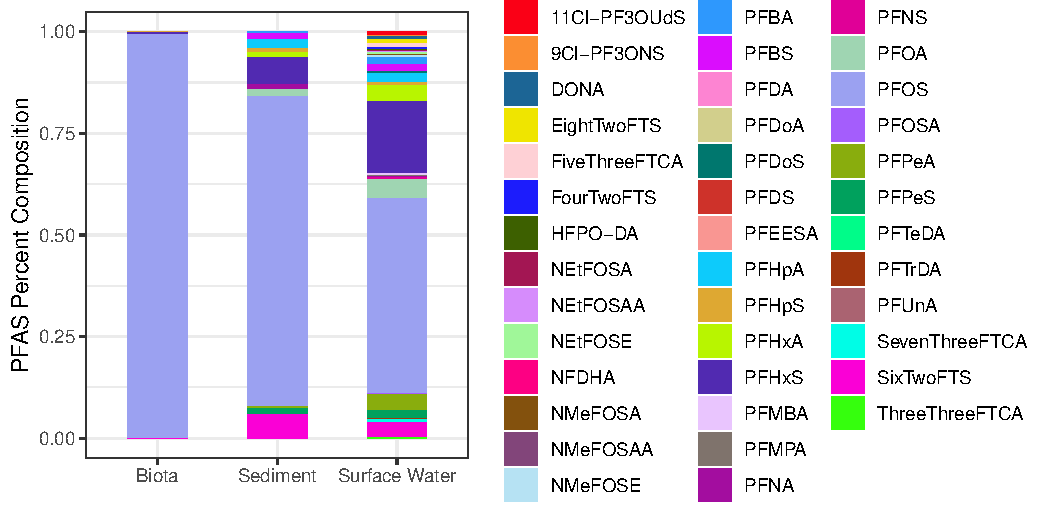
\includegraphics{CompleteDatasets_rerun_files/figure-latex/Figure 2 WG-1} 

}

\caption{Figure 2 (ms) WG}\label{fig:Figure 2 WG}
\end{figure}

\begin{Shaded}
\begin{Highlighting}[]
\CommentTok{\# ggsave(plot = fig2\_all, filename = "./Figures/SERDP/Fig2\_wg.png", height = 3.5, width = 8,units = "in")}
\CommentTok{\# fig2\_new}
\end{Highlighting}
\end{Shaded}

\begin{Shaded}
\begin{Highlighting}[]
\NormalTok{fig2\_all}\OtherTok{\textless{}{-}}\FunctionTok{ggplot}\NormalTok{(}\FunctionTok{rbind}\NormalTok{(d\_jba\_wat\_noSum,}
\NormalTok{                       d\_jba\_sed\_noSum,}
\NormalTok{                       d\_jba\_biota\_noSum,}
\NormalTok{                       d\_jba\_wat\_2024),}
       \FunctionTok{aes}\NormalTok{(}\AttributeTok{x=}\NormalTok{Media, }\AttributeTok{y=}\NormalTok{value, }\AttributeTok{fill=}\NormalTok{Analyte)) }\SpecialCharTok{+} 
  \FunctionTok{geom\_bar}\NormalTok{(}\AttributeTok{position=}\StringTok{\textquotesingle{}fill\textquotesingle{}}\NormalTok{, }\AttributeTok{width =} \FloatTok{0.5}\NormalTok{, }\AttributeTok{stat=}\StringTok{\textquotesingle{}identity\textquotesingle{}}\NormalTok{) }\SpecialCharTok{+}
  \FunctionTok{xlab}\NormalTok{(}\StringTok{""}\NormalTok{) }\SpecialCharTok{+}
  \FunctionTok{scale\_fill\_manual}\NormalTok{(}\AttributeTok{values =}\NormalTok{ P50)}\SpecialCharTok{+}
  \FunctionTok{ylab}\NormalTok{(}\StringTok{"PFAS Percent Composition"}\NormalTok{) }\SpecialCharTok{+}
  \FunctionTok{theme\_bw}\NormalTok{()}\SpecialCharTok{+}
  \FunctionTok{guides}\NormalTok{(}\AttributeTok{fill=}\FunctionTok{guide\_legend}\NormalTok{(}\AttributeTok{ncol=}\DecValTok{3}\NormalTok{))}
\CommentTok{\# fig2\_all}

\NormalTok{fig2\_new}\OtherTok{\textless{}{-}}\FunctionTok{ggplot}\NormalTok{(}\FunctionTok{rbind}\NormalTok{(d\_jba\_wat\_2024),}
       \FunctionTok{aes}\NormalTok{(}\AttributeTok{x=}\NormalTok{Media, }\AttributeTok{y=}\NormalTok{value, }\AttributeTok{fill=}\NormalTok{Analyte)) }\SpecialCharTok{+} 
  \FunctionTok{geom\_bar}\NormalTok{(}\AttributeTok{position=}\StringTok{\textquotesingle{}fill\textquotesingle{}}\NormalTok{, }\AttributeTok{width =} \FloatTok{0.5}\NormalTok{, }\AttributeTok{stat=}\StringTok{\textquotesingle{}identity\textquotesingle{}}\NormalTok{) }\SpecialCharTok{+}
  \FunctionTok{xlab}\NormalTok{(}\StringTok{""}\NormalTok{) }\SpecialCharTok{+}
  \FunctionTok{scale\_fill\_manual}\NormalTok{(}\AttributeTok{values =}\NormalTok{ P50)}\SpecialCharTok{+}
  \FunctionTok{ylab}\NormalTok{(}\StringTok{"PFAS Percent Composition"}\NormalTok{) }\SpecialCharTok{+}
  \FunctionTok{theme\_bw}\NormalTok{()}\SpecialCharTok{+}
  \FunctionTok{guides}\NormalTok{(}\AttributeTok{fill=}\FunctionTok{guide\_legend}\NormalTok{(}\AttributeTok{ncol=}\DecValTok{3}\NormalTok{))}

\NormalTok{fig2\_all}
\end{Highlighting}
\end{Shaded}

\begin{figure}

{\centering 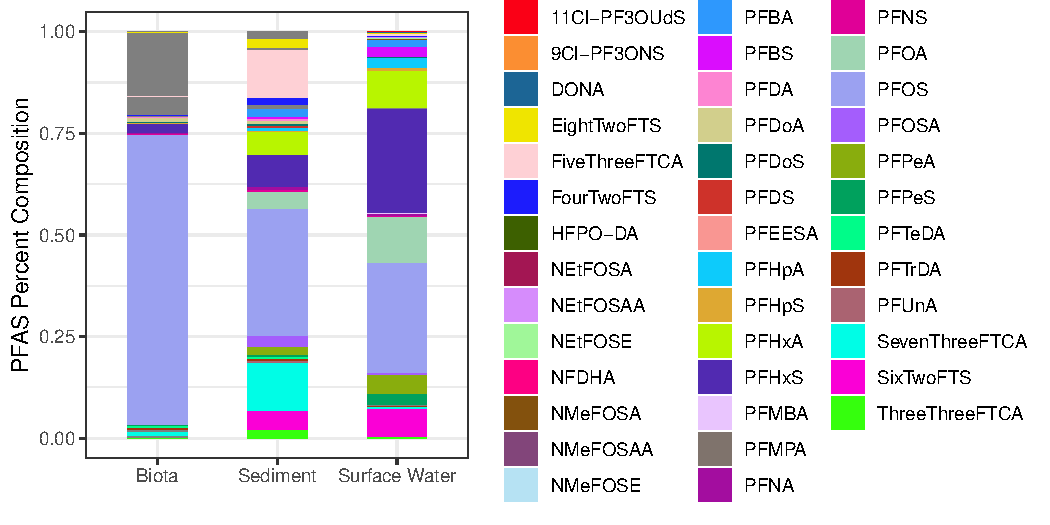
\includegraphics{CompleteDatasets_rerun_files/figure-latex/Figure 2 JBA-1} 

}

\caption{Figure 2 (ms) JBA}\label{fig:Figure 2 JBA}
\end{figure}

\begin{Shaded}
\begin{Highlighting}[]
\CommentTok{\# fig2\_new}
\CommentTok{\# ggsave(plot = fig2\_all, filename = "./Figures/SERDP/Fig2\_jba.png", height = 3.5, width = 8,units = "in")}
\end{Highlighting}
\end{Shaded}

\subsection{Figure 3 (Brown et al
2023)}\label{figure-3-brown-et-al-2023}

Abbi: This plot should be the line chart with the 4 sampling locations
and sum PFAS surface water concentrations over time (Figure 3 in the
paper). For this one I inserted the second y axis and scaled it to the
data (Not sure if you know what I mean, but if you can start with
recreating the line plot I can add the second y axis because I can't
find that code right now so i'll have to re-do it, but here's code to
start!)

\textbf{TASKS/QUESTIONS}:

\begin{itemize}
\tightlist
\item
  Pick a color scheme?
\item
  Biota - is a specific tissue plotted?
\end{itemize}

\begin{Shaded}
\begin{Highlighting}[]
\CommentTok{\# get data first summarise sum PFAS by date}
\NormalTok{p.full}\OtherTok{\textless{}{-}}\FunctionTok{rbind}\NormalTok{(d\_wg\_wat\_noSum, d\_wg\_wat\_2024) }\SpecialCharTok{\%\textgreater{}\%} 
  \FunctionTok{mutate}\NormalTok{(}\AttributeTok{SampleID =} \FunctionTok{factor}\NormalTok{(SampleID)) }\SpecialCharTok{\%\textgreater{}\%} 
\NormalTok{  dplyr}\SpecialCharTok{::}\FunctionTok{group\_by}\NormalTok{(SampleID, Spp\_Loc, Media, SampleDate) }\SpecialCharTok{\%\textgreater{}\%} 
\NormalTok{  dplyr}\SpecialCharTok{::}\FunctionTok{summarise}\NormalTok{(}\AttributeTok{SumPFAS =} \FunctionTok{sum}\NormalTok{(value, }\AttributeTok{na.rm =}\NormalTok{ T)) }\SpecialCharTok{\%\textgreater{}\%} 
  \FunctionTok{ggplot}\NormalTok{(}\FunctionTok{aes}\NormalTok{(}\AttributeTok{x=}\FunctionTok{as.Date}\NormalTok{(SampleDate), }\AttributeTok{y=}\NormalTok{SumPFAS, }\AttributeTok{group=}\NormalTok{Spp\_Loc, }\AttributeTok{color=}\NormalTok{Spp\_Loc)) }\SpecialCharTok{+}
    \FunctionTok{annotate}\NormalTok{(}\StringTok{"rect"}\NormalTok{, }\AttributeTok{xmin =} \FunctionTok{as.Date}\NormalTok{(}\StringTok{"2020{-}10{-}1"}\NormalTok{), }\AttributeTok{xmax =} \FunctionTok{as.Date}\NormalTok{(}\StringTok{"2020{-}11{-}20"}\NormalTok{),}
             \AttributeTok{ymin =} \SpecialCharTok{{-}}\ConstantTok{Inf}\NormalTok{, }\AttributeTok{ymax =} \ConstantTok{Inf}\NormalTok{,}
             \AttributeTok{alpha =}\NormalTok{ .}\DecValTok{1}\NormalTok{, }\AttributeTok{fill =} \StringTok{"black"}\NormalTok{)}\SpecialCharTok{+}
    \FunctionTok{annotate}\NormalTok{(}\StringTok{"rect"}\NormalTok{, }\AttributeTok{xmin =} \FunctionTok{as.Date}\NormalTok{(}\StringTok{"2021{-}01{-}30"}\NormalTok{), }\AttributeTok{xmax =} \FunctionTok{as.Date}\NormalTok{(}\StringTok{"2021{-}04{-}01"}\NormalTok{),}
             \AttributeTok{ymin =} \SpecialCharTok{{-}}\ConstantTok{Inf}\NormalTok{, }\AttributeTok{ymax =} \ConstantTok{Inf}\NormalTok{,}
             \AttributeTok{alpha =}\NormalTok{ .}\DecValTok{1}\NormalTok{, }\AttributeTok{fill =} \StringTok{"black"}\NormalTok{)}\SpecialCharTok{+}
    \FunctionTok{annotate}\NormalTok{(}\StringTok{"rect"}\NormalTok{, }\AttributeTok{xmin =} \FunctionTok{as.Date}\NormalTok{(}\StringTok{"2021{-}06{-}01"}\NormalTok{), }\AttributeTok{xmax =} \FunctionTok{as.Date}\NormalTok{(}\StringTok{"2021{-}07{-}30"}\NormalTok{),}
             \AttributeTok{ymin =} \SpecialCharTok{{-}}\ConstantTok{Inf}\NormalTok{, }\AttributeTok{ymax =} \ConstantTok{Inf}\NormalTok{,}
             \AttributeTok{alpha =}\NormalTok{ .}\DecValTok{1}\NormalTok{, }\AttributeTok{fill =} \StringTok{"black"}\NormalTok{)}\SpecialCharTok{+}\CommentTok{\# geom\_line(alpha = 0.3)+}
    \FunctionTok{geom\_point}\NormalTok{(}\AttributeTok{size=}\FloatTok{0.5}\NormalTok{)}\SpecialCharTok{+}
    \FunctionTok{ylab}\NormalTok{(}\StringTok{"Sum PFAS Concentration (ng/L)"}\NormalTok{) }\SpecialCharTok{+}
    \FunctionTok{xlab}\NormalTok{(}\StringTok{""}\NormalTok{)}\SpecialCharTok{+}
    \FunctionTok{scale\_color\_aaas}\NormalTok{()}\SpecialCharTok{+}
    \FunctionTok{scale\_y\_continuous}\NormalTok{(}\AttributeTok{breaks=}\FunctionTok{c}\NormalTok{(}\DecValTok{500}\NormalTok{,}\DecValTok{1000}\NormalTok{,}\DecValTok{1500}\NormalTok{,}\DecValTok{2000}\NormalTok{,}\DecValTok{2500}\NormalTok{, }\DecValTok{3000}\NormalTok{, }\DecValTok{3500}\NormalTok{)) }\SpecialCharTok{+}
    \FunctionTok{scale\_x\_date}\NormalTok{(}\AttributeTok{date\_labels =} \StringTok{"\%b \%d"}\NormalTok{, }\AttributeTok{breaks =} \StringTok{"2 months"}\NormalTok{)}\SpecialCharTok{+}
    \FunctionTok{theme\_bw}\NormalTok{()}\SpecialCharTok{+}
    \FunctionTok{theme}\NormalTok{(}\AttributeTok{axis.text.x =} \FunctionTok{element\_text}\NormalTok{(}\AttributeTok{angle =} \DecValTok{45}\NormalTok{, }\AttributeTok{hjust=}\DecValTok{1}\NormalTok{),}
          \AttributeTok{panel.grid.minor =} \FunctionTok{element\_blank}\NormalTok{())}

\NormalTok{p.A}\OtherTok{\textless{}{-}}\FunctionTok{rbind}\NormalTok{(d\_wg\_wat\_2024) }\SpecialCharTok{\%\textgreater{}\%}
  \FunctionTok{mutate}\NormalTok{(}\AttributeTok{SampleID =} \FunctionTok{factor}\NormalTok{(SampleID)) }\SpecialCharTok{\%\textgreater{}\%}
\NormalTok{  dplyr}\SpecialCharTok{::}\FunctionTok{group\_by}\NormalTok{(SampleID, Spp\_Loc, Media, SampleDate) }\SpecialCharTok{\%\textgreater{}\%}
\NormalTok{  dplyr}\SpecialCharTok{::}\FunctionTok{summarise}\NormalTok{(}\AttributeTok{SumPFAS =} \FunctionTok{sum}\NormalTok{(value, }\AttributeTok{na.rm =}\NormalTok{ T)) }\SpecialCharTok{\%\textgreater{}\%}
  \FunctionTok{filter}\NormalTok{(SampleDate }\SpecialCharTok{\textgreater{}} \FunctionTok{as.Date}\NormalTok{(}\StringTok{"2021{-}01{-}30"}\NormalTok{) }\SpecialCharTok{\&}\NormalTok{ SampleDate }\SpecialCharTok{\textless{}} \FunctionTok{as.Date}\NormalTok{(}\StringTok{"2021{-}04{-}01"}\NormalTok{)) }\SpecialCharTok{\%\textgreater{}\%}     \FunctionTok{ggplot}\NormalTok{(}\FunctionTok{aes}\NormalTok{(}\AttributeTok{x=}\FunctionTok{as.Date}\NormalTok{(SampleDate), }\AttributeTok{y=}\NormalTok{SumPFAS, }\AttributeTok{group=}\NormalTok{Spp\_Loc, }\AttributeTok{color=}\NormalTok{Spp\_Loc)) }\SpecialCharTok{+}
    \FunctionTok{geom\_line}\NormalTok{()}\SpecialCharTok{+}
    \FunctionTok{geom\_point}\NormalTok{(}\AttributeTok{size=}\FloatTok{0.5}\NormalTok{)}\SpecialCharTok{+}
    \FunctionTok{ylab}\NormalTok{(}\StringTok{"Sum PFAS Concentration (ng/L)"}\NormalTok{) }\SpecialCharTok{+}
    \FunctionTok{xlab}\NormalTok{(}\StringTok{""}\NormalTok{)}\SpecialCharTok{+}
    \FunctionTok{scale\_y\_continuous}\NormalTok{(}\AttributeTok{breaks=}\FunctionTok{c}\NormalTok{(}\DecValTok{500}\NormalTok{,}\DecValTok{1000}\NormalTok{,}\DecValTok{1500}\NormalTok{,}\DecValTok{2000}\NormalTok{,}\DecValTok{2500}\NormalTok{, }\DecValTok{3000}\NormalTok{, }\DecValTok{3500}\NormalTok{)) }\SpecialCharTok{+}
    \FunctionTok{scale\_x\_date}\NormalTok{(}\AttributeTok{date\_labels =} \StringTok{"\%b \%d"}\NormalTok{, }\AttributeTok{breaks =} \StringTok{"1 week"}\NormalTok{)}\SpecialCharTok{+}
    \FunctionTok{scale\_color\_aaas}\NormalTok{()}\SpecialCharTok{+}
    \FunctionTok{theme\_bw}\NormalTok{()}\SpecialCharTok{+}
    \FunctionTok{theme}\NormalTok{(}\AttributeTok{axis.text.x =} \FunctionTok{element\_text}\NormalTok{(}\AttributeTok{angle =} \DecValTok{45}\NormalTok{, }\AttributeTok{hjust=}\DecValTok{1}\NormalTok{),}
          \AttributeTok{panel.grid.minor =} \FunctionTok{element\_blank}\NormalTok{(),}
          \AttributeTok{legend.position =} \StringTok{"none"}\NormalTok{)}


\NormalTok{p.B}\OtherTok{\textless{}{-}}\FunctionTok{rbind}\NormalTok{(d\_wg\_wat\_2024) }\SpecialCharTok{\%\textgreater{}\%}
  \FunctionTok{mutate}\NormalTok{(}\AttributeTok{SampleID =} \FunctionTok{factor}\NormalTok{(SampleID)) }\SpecialCharTok{\%\textgreater{}\%}
\NormalTok{  dplyr}\SpecialCharTok{::}\FunctionTok{group\_by}\NormalTok{(SampleID, Spp\_Loc, Media, SampleDate) }\SpecialCharTok{\%\textgreater{}\%}
\NormalTok{  dplyr}\SpecialCharTok{::}\FunctionTok{summarise}\NormalTok{(}\AttributeTok{SumPFAS =} \FunctionTok{sum}\NormalTok{(value, }\AttributeTok{na.rm =}\NormalTok{ T)) }\SpecialCharTok{\%\textgreater{}\%}
  \FunctionTok{filter}\NormalTok{(SampleDate }\SpecialCharTok{\textgreater{}} \FunctionTok{as.Date}\NormalTok{(}\StringTok{"2021{-}06{-}01"}\NormalTok{) }\SpecialCharTok{\&}\NormalTok{ SampleDate }\SpecialCharTok{\textless{}} \FunctionTok{as.Date}\NormalTok{(}\StringTok{"2021{-}07{-}30"}\NormalTok{)) }\SpecialCharTok{\%\textgreater{}\%} 
    \FunctionTok{ggplot}\NormalTok{(}\FunctionTok{aes}\NormalTok{(}\AttributeTok{x=}\FunctionTok{as.Date}\NormalTok{(SampleDate), }\AttributeTok{y=}\NormalTok{SumPFAS, }\AttributeTok{group=}\NormalTok{Spp\_Loc, }\AttributeTok{color=}\NormalTok{Spp\_Loc)) }\SpecialCharTok{+}
    \FunctionTok{geom\_line}\NormalTok{()}\SpecialCharTok{+}
    \FunctionTok{geom\_point}\NormalTok{(}\AttributeTok{size=}\FloatTok{0.5}\NormalTok{)}\SpecialCharTok{+}
    \FunctionTok{ylab}\NormalTok{(}\StringTok{"Sum PFAS Concentration (ng/L)"}\NormalTok{) }\SpecialCharTok{+}
    \FunctionTok{xlab}\NormalTok{(}\StringTok{""}\NormalTok{)}\SpecialCharTok{+}
    \FunctionTok{scale\_color\_aaas}\NormalTok{()}\SpecialCharTok{+}
    \FunctionTok{scale\_y\_continuous}\NormalTok{(}\AttributeTok{breaks=}\FunctionTok{c}\NormalTok{(}\DecValTok{500}\NormalTok{,}\DecValTok{1000}\NormalTok{,}\DecValTok{1500}\NormalTok{,}\DecValTok{2000}\NormalTok{,}\DecValTok{2500}\NormalTok{, }\DecValTok{3000}\NormalTok{, }\DecValTok{3500}\NormalTok{)) }\SpecialCharTok{+}
    \FunctionTok{scale\_x\_date}\NormalTok{(}\AttributeTok{date\_labels =} \StringTok{"\%b \%d"}\NormalTok{, }\AttributeTok{breaks =} \StringTok{"1 week"}\NormalTok{)}\SpecialCharTok{+}
    \FunctionTok{theme\_bw}\NormalTok{()}\SpecialCharTok{+}
    \FunctionTok{theme}\NormalTok{(}\AttributeTok{axis.text.x =} \FunctionTok{element\_text}\NormalTok{(}\AttributeTok{angle =} \DecValTok{45}\NormalTok{, }\AttributeTok{hjust=}\DecValTok{1}\NormalTok{),}
          \AttributeTok{panel.grid.minor =} \FunctionTok{element\_blank}\NormalTok{(),}
          \AttributeTok{legend.position =} \StringTok{"none"}\NormalTok{)}


\NormalTok{p.C}\OtherTok{\textless{}{-}}\FunctionTok{rbind}\NormalTok{(d\_wg\_wat\_noSum) }\SpecialCharTok{\%\textgreater{}\%} 
  \FunctionTok{mutate}\NormalTok{(}\AttributeTok{SampleID =} \FunctionTok{factor}\NormalTok{(SampleID)) }\SpecialCharTok{\%\textgreater{}\%} 
\NormalTok{  dplyr}\SpecialCharTok{::}\FunctionTok{group\_by}\NormalTok{(SampleID, Spp\_Loc, Media, SampleDate) }\SpecialCharTok{\%\textgreater{}\%} 
\NormalTok{  dplyr}\SpecialCharTok{::}\FunctionTok{summarise}\NormalTok{(}\AttributeTok{SumPFAS =} \FunctionTok{sum}\NormalTok{(value, }\AttributeTok{na.rm =}\NormalTok{ T)) }\SpecialCharTok{\%\textgreater{}\%} 
    \FunctionTok{ggplot}\NormalTok{(}\FunctionTok{aes}\NormalTok{(}\AttributeTok{x=}\FunctionTok{as.Date}\NormalTok{(SampleDate), }\AttributeTok{y=}\NormalTok{SumPFAS, }\AttributeTok{group=}\NormalTok{Spp\_Loc, }\AttributeTok{color=}\NormalTok{Spp\_Loc)) }\SpecialCharTok{+}
    \FunctionTok{geom\_line}\NormalTok{()}\SpecialCharTok{+}
    \FunctionTok{geom\_point}\NormalTok{(}\AttributeTok{size=}\FloatTok{0.5}\NormalTok{)}\SpecialCharTok{+}
    \FunctionTok{ylab}\NormalTok{(}\StringTok{"Sum PFAS Concentration (ng/L)"}\NormalTok{) }\SpecialCharTok{+}
    \FunctionTok{xlab}\NormalTok{(}\StringTok{""}\NormalTok{)}\SpecialCharTok{+}
    \FunctionTok{scale\_color\_aaas}\NormalTok{()}\SpecialCharTok{+}
    \FunctionTok{scale\_y\_continuous}\NormalTok{(}\AttributeTok{breaks=}\FunctionTok{c}\NormalTok{(}\DecValTok{500}\NormalTok{,}\DecValTok{1000}\NormalTok{,}\DecValTok{1500}\NormalTok{,}\DecValTok{2000}\NormalTok{,}\DecValTok{2500}\NormalTok{, }\DecValTok{3000}\NormalTok{, }\DecValTok{3500}\NormalTok{)) }\SpecialCharTok{+}
    \FunctionTok{scale\_x\_date}\NormalTok{(}\AttributeTok{date\_labels =} \StringTok{"\%b \%d"}\NormalTok{, }\AttributeTok{breaks =} \StringTok{"1 week"}\NormalTok{)}\SpecialCharTok{+}
    \FunctionTok{theme\_bw}\NormalTok{()}\SpecialCharTok{+}
    \FunctionTok{theme}\NormalTok{(}\AttributeTok{axis.text.x =} \FunctionTok{element\_text}\NormalTok{(}\AttributeTok{angle =} \DecValTok{45}\NormalTok{, }\AttributeTok{hjust=}\DecValTok{1}\NormalTok{),}
          \AttributeTok{panel.grid.minor =} \FunctionTok{element\_blank}\NormalTok{(),}
          \AttributeTok{legend.position =} \StringTok{"none"}\NormalTok{)}

\NormalTok{row2}\OtherTok{\textless{}{-}}\NormalTok{cowplot}\SpecialCharTok{::}\FunctionTok{plot\_grid}\NormalTok{(p.C, p.A, p.B,  }
                   \AttributeTok{labels =} \FunctionTok{c}\NormalTok{(}\StringTok{"B"}\NormalTok{, }\StringTok{"C"}\NormalTok{, }\StringTok{"D"}\NormalTok{),}
                   \AttributeTok{nrow =} \DecValTok{1}\NormalTok{)}
\NormalTok{fig3}\OtherTok{\textless{}{-}}\NormalTok{cowplot}\SpecialCharTok{::}\FunctionTok{plot\_grid}\NormalTok{(p.full, row2, }
                   \AttributeTok{labels =} \FunctionTok{c}\NormalTok{(}\StringTok{"A"}\NormalTok{, }\StringTok{""}\NormalTok{),}
                   \AttributeTok{nrow =} \DecValTok{2}\NormalTok{)}

\CommentTok{\# ggsave(plot = fig3, filename = "./Figures/SERDP/Fig3\_wg.png",}
\CommentTok{\#        height = 7, width = 10,}
\CommentTok{\#        units = "in")}
\end{Highlighting}
\end{Shaded}

\begin{Shaded}
\begin{Highlighting}[]
\CommentTok{\# get data first summarise sum PFAS by date}
\NormalTok{p.full}\OtherTok{\textless{}{-}}
  \FunctionTok{rbind}\NormalTok{(d\_jba\_wat\_noSum, d\_jba\_wat\_2024) }\SpecialCharTok{\%\textgreater{}\%} 
  \FunctionTok{mutate}\NormalTok{(}\AttributeTok{SampleID =} \FunctionTok{factor}\NormalTok{(SampleID)) }\SpecialCharTok{\%\textgreater{}\%} 
\NormalTok{  dplyr}\SpecialCharTok{::}\FunctionTok{group\_by}\NormalTok{(SampleID, Spp\_Loc, Media, SampleDate) }\SpecialCharTok{\%\textgreater{}\%} 
\NormalTok{  dplyr}\SpecialCharTok{::}\FunctionTok{summarise}\NormalTok{(}\AttributeTok{SumPFAS =} \FunctionTok{sum}\NormalTok{(value, }\AttributeTok{na.rm =}\NormalTok{ T)) }\SpecialCharTok{\%\textgreater{}\%} 
  \FunctionTok{ggplot}\NormalTok{(}\FunctionTok{aes}\NormalTok{(}\AttributeTok{x=}\FunctionTok{as.Date}\NormalTok{(SampleDate), }\AttributeTok{y=}\NormalTok{SumPFAS, }\AttributeTok{group=}\NormalTok{Spp\_Loc, }\AttributeTok{color=}\NormalTok{Spp\_Loc)) }\SpecialCharTok{+}
    \FunctionTok{annotate}\NormalTok{(}\StringTok{"rect"}\NormalTok{, }\AttributeTok{xmin =} \FunctionTok{as.Date}\NormalTok{(}\StringTok{"2020{-}11{-}10"}\NormalTok{), }\AttributeTok{xmax =} \FunctionTok{as.Date}\NormalTok{(}\StringTok{"2020{-}12{-}25"}\NormalTok{),}
             \AttributeTok{ymin =} \SpecialCharTok{{-}}\ConstantTok{Inf}\NormalTok{, }\AttributeTok{ymax =} \ConstantTok{Inf}\NormalTok{,}
             \AttributeTok{alpha =}\NormalTok{ .}\DecValTok{1}\NormalTok{, }\AttributeTok{fill =} \StringTok{"black"}\NormalTok{)}\SpecialCharTok{+}
    \FunctionTok{annotate}\NormalTok{(}\StringTok{"rect"}\NormalTok{, }\AttributeTok{xmin =} \FunctionTok{as.Date}\NormalTok{(}\StringTok{"2021{-}03{-}28"}\NormalTok{), }\AttributeTok{xmax =} \FunctionTok{as.Date}\NormalTok{(}\StringTok{"2021{-}05{-}01"}\NormalTok{),}
             \AttributeTok{ymin =} \SpecialCharTok{{-}}\ConstantTok{Inf}\NormalTok{, }\AttributeTok{ymax =} \ConstantTok{Inf}\NormalTok{,}
             \AttributeTok{alpha =}\NormalTok{ .}\DecValTok{1}\NormalTok{, }\AttributeTok{fill =} \StringTok{"black"}\NormalTok{)}\SpecialCharTok{+}
    \FunctionTok{annotate}\NormalTok{(}\StringTok{"rect"}\NormalTok{, }\AttributeTok{xmin =} \FunctionTok{as.Date}\NormalTok{(}\StringTok{"2021{-}06{-}10"}\NormalTok{), }\AttributeTok{xmax =} \FunctionTok{as.Date}\NormalTok{(}\StringTok{"2021{-}07{-}20"}\NormalTok{),}
             \AttributeTok{ymin =} \SpecialCharTok{{-}}\ConstantTok{Inf}\NormalTok{, }\AttributeTok{ymax =} \ConstantTok{Inf}\NormalTok{,}
             \AttributeTok{alpha =}\NormalTok{ .}\DecValTok{1}\NormalTok{, }\AttributeTok{fill =} \StringTok{"black"}\NormalTok{)}\SpecialCharTok{+}\CommentTok{\# geom\_line(alpha = 0.3)+}
    \FunctionTok{geom\_point}\NormalTok{(}\AttributeTok{size=}\FloatTok{0.5}\NormalTok{)}\SpecialCharTok{+}
    \FunctionTok{ylab}\NormalTok{(}\StringTok{"Sum PFAS Concentration (ng/L)"}\NormalTok{) }\SpecialCharTok{+}
    \FunctionTok{xlab}\NormalTok{(}\StringTok{""}\NormalTok{)}\SpecialCharTok{+}
    \FunctionTok{scale\_color\_aaas}\NormalTok{()}\SpecialCharTok{+}
    \FunctionTok{scale\_y\_continuous}\NormalTok{(}\AttributeTok{breaks=}\FunctionTok{c}\NormalTok{(}\FunctionTok{seq}\NormalTok{(}\DecValTok{500}\NormalTok{,}\DecValTok{8000}\NormalTok{, }\DecValTok{500}\NormalTok{))) }\SpecialCharTok{+}
    \FunctionTok{scale\_x\_date}\NormalTok{(}\AttributeTok{date\_labels =} \StringTok{"\%b \%d"}\NormalTok{, }\AttributeTok{breaks =} \StringTok{"2 months"}\NormalTok{)}\SpecialCharTok{+}
    \FunctionTok{theme\_bw}\NormalTok{()}\SpecialCharTok{+}
    \FunctionTok{theme}\NormalTok{(}\AttributeTok{axis.text.x =} \FunctionTok{element\_text}\NormalTok{(}\AttributeTok{angle =} \DecValTok{45}\NormalTok{, }\AttributeTok{hjust=}\DecValTok{1}\NormalTok{),}
          \AttributeTok{panel.grid.minor =} \FunctionTok{element\_blank}\NormalTok{())}

\NormalTok{p.A}\OtherTok{\textless{}{-}}\FunctionTok{rbind}\NormalTok{(d\_jba\_wat\_noSum, d\_jba\_wat\_2024) }\SpecialCharTok{\%\textgreater{}\%}
  \FunctionTok{mutate}\NormalTok{(}\AttributeTok{SampleID =} \FunctionTok{factor}\NormalTok{(SampleID)) }\SpecialCharTok{\%\textgreater{}\%}
\NormalTok{  dplyr}\SpecialCharTok{::}\FunctionTok{group\_by}\NormalTok{(SampleID, Spp\_Loc, Media, SampleDate) }\SpecialCharTok{\%\textgreater{}\%}
\NormalTok{  dplyr}\SpecialCharTok{::}\FunctionTok{summarise}\NormalTok{(}\AttributeTok{SumPFAS =} \FunctionTok{sum}\NormalTok{(value, }\AttributeTok{na.rm =}\NormalTok{ T)) }\SpecialCharTok{\%\textgreater{}\%}
  \FunctionTok{filter}\NormalTok{(SampleDate }\SpecialCharTok{\textgreater{}} \FunctionTok{as.Date}\NormalTok{(}\StringTok{"2020{-}11{-}10"}\NormalTok{) }\SpecialCharTok{\&}\NormalTok{ SampleDate }\SpecialCharTok{\textless{}} \FunctionTok{as.Date}\NormalTok{(}\StringTok{"2020{-}12{-}25"}\NormalTok{)) }\SpecialCharTok{\%\textgreater{}\%}     \FunctionTok{ggplot}\NormalTok{(}\FunctionTok{aes}\NormalTok{(}\AttributeTok{x=}\FunctionTok{as.Date}\NormalTok{(SampleDate), }\AttributeTok{y=}\NormalTok{SumPFAS, }\AttributeTok{group=}\NormalTok{Spp\_Loc, }\AttributeTok{color=}\NormalTok{Spp\_Loc)) }\SpecialCharTok{+}
    \FunctionTok{geom\_line}\NormalTok{()}\SpecialCharTok{+}
    \FunctionTok{geom\_point}\NormalTok{(}\AttributeTok{size=}\FloatTok{0.5}\NormalTok{)}\SpecialCharTok{+}
    \FunctionTok{ylab}\NormalTok{(}\StringTok{"Sum PFAS Concentration (ng/L)"}\NormalTok{) }\SpecialCharTok{+}
    \FunctionTok{xlab}\NormalTok{(}\StringTok{""}\NormalTok{)}\SpecialCharTok{+}
    \FunctionTok{scale\_y\_continuous}\NormalTok{(}\AttributeTok{breaks=}\FunctionTok{c}\NormalTok{(}\FunctionTok{seq}\NormalTok{(}\DecValTok{500}\NormalTok{,}\DecValTok{8000}\NormalTok{, }\DecValTok{500}\NormalTok{))) }\SpecialCharTok{+}
    \FunctionTok{scale\_x\_date}\NormalTok{(}\AttributeTok{date\_labels =} \StringTok{"\%b \%d"}\NormalTok{, }\AttributeTok{breaks =} \StringTok{"1 week"}\NormalTok{)}\SpecialCharTok{+}
    \FunctionTok{scale\_color\_aaas}\NormalTok{()}\SpecialCharTok{+}
    \FunctionTok{theme\_bw}\NormalTok{()}\SpecialCharTok{+}
    \FunctionTok{theme}\NormalTok{(}\AttributeTok{axis.text.x =} \FunctionTok{element\_text}\NormalTok{(}\AttributeTok{angle =} \DecValTok{45}\NormalTok{, }\AttributeTok{hjust=}\DecValTok{1}\NormalTok{),}
          \AttributeTok{panel.grid.minor =} \FunctionTok{element\_blank}\NormalTok{(),}
          \AttributeTok{legend.position =} \StringTok{"none"}\NormalTok{)}


\NormalTok{p.B}\OtherTok{\textless{}{-}}\FunctionTok{rbind}\NormalTok{(d\_jba\_wat\_noSum, d\_jba\_wat\_2024) }\SpecialCharTok{\%\textgreater{}\%}
  \FunctionTok{mutate}\NormalTok{(}\AttributeTok{SampleID =} \FunctionTok{factor}\NormalTok{(SampleID)) }\SpecialCharTok{\%\textgreater{}\%}
\NormalTok{  dplyr}\SpecialCharTok{::}\FunctionTok{group\_by}\NormalTok{(SampleID, Spp\_Loc, Media, SampleDate) }\SpecialCharTok{\%\textgreater{}\%}
\NormalTok{  dplyr}\SpecialCharTok{::}\FunctionTok{summarise}\NormalTok{(}\AttributeTok{SumPFAS =} \FunctionTok{sum}\NormalTok{(value, }\AttributeTok{na.rm =}\NormalTok{ T)) }\SpecialCharTok{\%\textgreater{}\%}
  \FunctionTok{filter}\NormalTok{(SampleDate }\SpecialCharTok{\textgreater{}} \FunctionTok{as.Date}\NormalTok{(}\StringTok{"2021{-}03{-}28"}\NormalTok{) }\SpecialCharTok{\&}\NormalTok{ SampleDate }\SpecialCharTok{\textless{}} \FunctionTok{as.Date}\NormalTok{(}\StringTok{"2021{-}05{-}01"}\NormalTok{)) }\SpecialCharTok{\%\textgreater{}\%} 
    \FunctionTok{ggplot}\NormalTok{(}\FunctionTok{aes}\NormalTok{(}\AttributeTok{x=}\FunctionTok{as.Date}\NormalTok{(SampleDate), }\AttributeTok{y=}\NormalTok{SumPFAS, }\AttributeTok{group=}\NormalTok{Spp\_Loc, }\AttributeTok{color=}\NormalTok{Spp\_Loc)) }\SpecialCharTok{+}
    \FunctionTok{geom\_line}\NormalTok{()}\SpecialCharTok{+}
    \FunctionTok{geom\_point}\NormalTok{(}\AttributeTok{size=}\FloatTok{0.5}\NormalTok{)}\SpecialCharTok{+}
    \FunctionTok{ylab}\NormalTok{(}\StringTok{"Sum PFAS Concentration (ng/L)"}\NormalTok{) }\SpecialCharTok{+}
    \FunctionTok{xlab}\NormalTok{(}\StringTok{""}\NormalTok{)}\SpecialCharTok{+}
    \FunctionTok{scale\_color\_aaas}\NormalTok{()}\SpecialCharTok{+}
    \FunctionTok{scale\_y\_continuous}\NormalTok{(}\AttributeTok{breaks=}\FunctionTok{c}\NormalTok{(}\FunctionTok{seq}\NormalTok{(}\DecValTok{500}\NormalTok{,}\DecValTok{8000}\NormalTok{, }\DecValTok{500}\NormalTok{))) }\SpecialCharTok{+}
    \FunctionTok{scale\_x\_date}\NormalTok{(}\AttributeTok{date\_labels =} \StringTok{"\%b \%d"}\NormalTok{, }\AttributeTok{breaks =} \StringTok{"1 week"}\NormalTok{)}\SpecialCharTok{+}
    \FunctionTok{theme\_bw}\NormalTok{()}\SpecialCharTok{+}
    \FunctionTok{theme}\NormalTok{(}\AttributeTok{axis.text.x =} \FunctionTok{element\_text}\NormalTok{(}\AttributeTok{angle =} \DecValTok{45}\NormalTok{, }\AttributeTok{hjust=}\DecValTok{1}\NormalTok{),}
          \AttributeTok{panel.grid.minor =} \FunctionTok{element\_blank}\NormalTok{(),}
          \AttributeTok{legend.position =} \StringTok{"none"}\NormalTok{)}

\NormalTok{p.C}\OtherTok{\textless{}{-}}\FunctionTok{rbind}\NormalTok{(d\_jba\_wat\_noSum, d\_jba\_wat\_2024) }\SpecialCharTok{\%\textgreater{}\%}
  \FunctionTok{mutate}\NormalTok{(}\AttributeTok{SampleID =} \FunctionTok{factor}\NormalTok{(SampleID)) }\SpecialCharTok{\%\textgreater{}\%}
\NormalTok{  dplyr}\SpecialCharTok{::}\FunctionTok{group\_by}\NormalTok{(SampleID, Spp\_Loc, Media, SampleDate) }\SpecialCharTok{\%\textgreater{}\%}
\NormalTok{  dplyr}\SpecialCharTok{::}\FunctionTok{summarise}\NormalTok{(}\AttributeTok{SumPFAS =} \FunctionTok{sum}\NormalTok{(value, }\AttributeTok{na.rm =}\NormalTok{ T)) }\SpecialCharTok{\%\textgreater{}\%}
  \FunctionTok{filter}\NormalTok{(SampleDate }\SpecialCharTok{\textgreater{}} \FunctionTok{as.Date}\NormalTok{(}\StringTok{"2021{-}06{-}10"}\NormalTok{) }\SpecialCharTok{\&}\NormalTok{ SampleDate }\SpecialCharTok{\textless{}} \FunctionTok{as.Date}\NormalTok{(}\StringTok{"2021{-}07{-}20"}\NormalTok{)) }\SpecialCharTok{\%\textgreater{}\%} 
    \FunctionTok{ggplot}\NormalTok{(}\FunctionTok{aes}\NormalTok{(}\AttributeTok{x=}\FunctionTok{as.Date}\NormalTok{(SampleDate), }\AttributeTok{y=}\NormalTok{SumPFAS, }\AttributeTok{group=}\NormalTok{Spp\_Loc, }\AttributeTok{color=}\NormalTok{Spp\_Loc)) }\SpecialCharTok{+}
    \FunctionTok{geom\_line}\NormalTok{()}\SpecialCharTok{+}
    \FunctionTok{geom\_point}\NormalTok{(}\AttributeTok{size=}\FloatTok{0.5}\NormalTok{)}\SpecialCharTok{+}
    \FunctionTok{ylab}\NormalTok{(}\StringTok{"Sum PFAS Concentration (ng/L)"}\NormalTok{) }\SpecialCharTok{+}
    \FunctionTok{xlab}\NormalTok{(}\StringTok{""}\NormalTok{)}\SpecialCharTok{+}
    \FunctionTok{scale\_color\_aaas}\NormalTok{()}\SpecialCharTok{+}
    \FunctionTok{scale\_y\_continuous}\NormalTok{(}\AttributeTok{breaks=}\FunctionTok{c}\NormalTok{(}\FunctionTok{seq}\NormalTok{(}\DecValTok{500}\NormalTok{,}\DecValTok{8000}\NormalTok{, }\DecValTok{500}\NormalTok{))) }\SpecialCharTok{+}
    \FunctionTok{scale\_x\_date}\NormalTok{(}\AttributeTok{date\_labels =} \StringTok{"\%b \%d"}\NormalTok{, }\AttributeTok{breaks =} \StringTok{"1 week"}\NormalTok{)}\SpecialCharTok{+}
    \FunctionTok{theme\_bw}\NormalTok{()}\SpecialCharTok{+}
    \FunctionTok{theme}\NormalTok{(}\AttributeTok{axis.text.x =} \FunctionTok{element\_text}\NormalTok{(}\AttributeTok{angle =} \DecValTok{45}\NormalTok{, }\AttributeTok{hjust=}\DecValTok{1}\NormalTok{),}
          \AttributeTok{panel.grid.minor =} \FunctionTok{element\_blank}\NormalTok{(),}
          \AttributeTok{legend.position =} \StringTok{"none"}\NormalTok{)}

\NormalTok{row2}\OtherTok{\textless{}{-}}\NormalTok{cowplot}\SpecialCharTok{::}\FunctionTok{plot\_grid}\NormalTok{(p.A, p.B, p.C,  }
                   \AttributeTok{labels =} \FunctionTok{c}\NormalTok{(}\StringTok{"B"}\NormalTok{, }\StringTok{"C"}\NormalTok{, }\StringTok{"D"}\NormalTok{),}
                   \AttributeTok{nrow =} \DecValTok{1}\NormalTok{)}
\NormalTok{fig3}\OtherTok{\textless{}{-}}\NormalTok{cowplot}\SpecialCharTok{::}\FunctionTok{plot\_grid}\NormalTok{(p.full, row2, }
                   \AttributeTok{labels =} \FunctionTok{c}\NormalTok{(}\StringTok{"A"}\NormalTok{, }\StringTok{""}\NormalTok{),}
                   \AttributeTok{nrow =} \DecValTok{2}\NormalTok{)}

\CommentTok{\# ggsave(plot = fig3, filename = "./Figures/SERDP/Fig3\_jba.png",}
\CommentTok{\#        height = 7, width = 10,}
\CommentTok{\#        units = "in")}
\end{Highlighting}
\end{Shaded}

\subsection{Figure 4 (Brown et al
2023)}\label{figure-4-brown-et-al-2023}

Abbi: This is for the heatmaps (Figure 4 in the paper). At the time I
just added the annotations in the PDF after creating the file, but now
I'd do them in R since i'm better at that now haha

\emph{TASKS/QUESTIONS}:

\begin{itemize}
\tightlist
\item
  What needs to be excluded (some PFAS are below the detection limit?)
\item
  No correlation done
\end{itemize}

\begin{Shaded}
\begin{Highlighting}[]
\NormalTok{df2}\OtherTok{\textless{}{-}}\FunctionTok{rbind}\NormalTok{(d\_wg\_wat\_noSum, d\_wg\_wat\_2024) }\SpecialCharTok{\%\textgreater{}\%} 
\NormalTok{  dplyr}\SpecialCharTok{::}\FunctionTok{group\_by}\NormalTok{(SampleDate, Analyte) }\SpecialCharTok{\%\textgreater{}\%} 
\NormalTok{  dplyr}\SpecialCharTok{::}\FunctionTok{summarise}\NormalTok{(}\AttributeTok{meanPFAS =} \FunctionTok{round}\NormalTok{(}\FunctionTok{mean}\NormalTok{(value, }\AttributeTok{na.rm =}\NormalTok{ T), }\DecValTok{1}\NormalTok{)) }\SpecialCharTok{\%\textgreater{}\%}
  \FunctionTok{mutate}\NormalTok{(}\AttributeTok{meanPFAS =} \FunctionTok{as.numeric}\NormalTok{(meanPFAS)) }\SpecialCharTok{\%\textgreater{}\%}
  \FunctionTok{pivot\_wider}\NormalTok{(}\AttributeTok{values\_from =} \StringTok{"meanPFAS"}\NormalTok{, }\AttributeTok{names\_from =} \StringTok{"Analyte"}\NormalTok{) }\SpecialCharTok{\%\textgreater{}\%} 
  \FunctionTok{as.data.frame}\NormalTok{()}

\FunctionTok{rownames}\NormalTok{(df2)}\OtherTok{\textless{}{-}}\NormalTok{df2}\SpecialCharTok{$}\NormalTok{SampleDate}
\NormalTok{df2}\OtherTok{\textless{}{-}}\FunctionTok{as.matrix}\NormalTok{(df2[,}\SpecialCharTok{{-}}\DecValTok{1}\NormalTok{])}

\FunctionTok{heatmaply}\NormalTok{(df2,}
              \AttributeTok{scale\_fill\_gradient\_fun =}\NormalTok{ ggplot2}\SpecialCharTok{::}\FunctionTok{scale\_fill\_gradientn}\NormalTok{(}
                \AttributeTok{colours =} \FunctionTok{c}\NormalTok{(}\StringTok{"darkgreen"}\NormalTok{,}\StringTok{"lightgreen"}\NormalTok{,}\StringTok{"yellow"}\NormalTok{,}\StringTok{"orange"}\NormalTok{,}\StringTok{"red"}\NormalTok{,}\StringTok{"darkred"}\NormalTok{)),}
              \AttributeTok{dendrogram =} \StringTok{"none"}\NormalTok{,}
              \AttributeTok{xlab =} \StringTok{""}\NormalTok{, }\AttributeTok{ylab =} \StringTok{""}\NormalTok{,}
              \AttributeTok{main =} \StringTok{""}\NormalTok{,}
              \AttributeTok{scale =} \StringTok{"column"}\NormalTok{,}
              \AttributeTok{margins =} \FunctionTok{c}\NormalTok{(}\DecValTok{40}\NormalTok{,}\DecValTok{80}\NormalTok{,}\DecValTok{10}\NormalTok{,}\DecValTok{10}\NormalTok{),}
              \AttributeTok{grid\_color =} \StringTok{"white"}\NormalTok{,}
              \AttributeTok{grid\_width =} \FloatTok{0.00001}\NormalTok{,}
              \AttributeTok{titleX =} \ConstantTok{FALSE}\NormalTok{,}
              \AttributeTok{hide\_colorbar =} \ConstantTok{FALSE}\NormalTok{,}
              \AttributeTok{cellnote =}\NormalTok{ df2,}
              \AttributeTok{cellnote\_textposition =} \StringTok{"middle center"}\NormalTok{,}
              \AttributeTok{cellnote\_size =} \DecValTok{8}\NormalTok{,}
              \AttributeTok{branches\_lwd =} \FloatTok{0.1}\NormalTok{,}
              \AttributeTok{fontsize\_row =} \DecValTok{10}\NormalTok{,}
              \AttributeTok{fontsize\_col =} \DecValTok{10}\NormalTok{,}
              \AttributeTok{labCol =} \FunctionTok{colnames}\NormalTok{(df2),}
              \AttributeTok{labRow =} \FunctionTok{rownames}\NormalTok{(df2),}
              \AttributeTok{heatmap\_layers =} \FunctionTok{theme}\NormalTok{(}\AttributeTok{axis.line=}\FunctionTok{element\_blank}\NormalTok{(),}
                                     \CommentTok{\# axis.text.x=element\_blank(),}
                                     \AttributeTok{axis.ticks.x=}\FunctionTok{element\_blank}\NormalTok{(),}
                                     \AttributeTok{axis.text.y=}\FunctionTok{element\_text}\NormalTok{(}\AttributeTok{size =} \DecValTok{12}\NormalTok{,}
                                                              \AttributeTok{color=}\StringTok{"black"}\NormalTok{,}
                                                              \AttributeTok{family =} \StringTok{"Times New Roman"}\NormalTok{))}
\NormalTok{)}

 \CommentTok{\# saved using screenshot..}
\end{Highlighting}
\end{Shaded}

\begin{Shaded}
\begin{Highlighting}[]
\NormalTok{df2}\OtherTok{\textless{}{-}}\FunctionTok{rbind}\NormalTok{(d\_jba\_wat\_noSum, d\_jba\_wat\_2024) }\SpecialCharTok{\%\textgreater{}\%} 
\NormalTok{  dplyr}\SpecialCharTok{::}\FunctionTok{group\_by}\NormalTok{(SampleDate, Analyte) }\SpecialCharTok{\%\textgreater{}\%} 
\NormalTok{  dplyr}\SpecialCharTok{::}\FunctionTok{summarise}\NormalTok{(}\AttributeTok{meanPFAS =} \FunctionTok{round}\NormalTok{(}\FunctionTok{mean}\NormalTok{(value, }\AttributeTok{na.rm =}\NormalTok{ T), }\DecValTok{1}\NormalTok{)) }\SpecialCharTok{\%\textgreater{}\%}
  \FunctionTok{mutate}\NormalTok{(}\AttributeTok{meanPFAS =} \FunctionTok{as.numeric}\NormalTok{(meanPFAS)) }\SpecialCharTok{\%\textgreater{}\%}
  \FunctionTok{pivot\_wider}\NormalTok{(}\AttributeTok{values\_from =} \StringTok{"meanPFAS"}\NormalTok{, }\AttributeTok{names\_from =} \StringTok{"Analyte"}\NormalTok{) }\SpecialCharTok{\%\textgreater{}\%} 
  \FunctionTok{as.data.frame}\NormalTok{()}
\FunctionTok{rownames}\NormalTok{(df2)}\OtherTok{\textless{}{-}}\NormalTok{df2}\SpecialCharTok{$}\NormalTok{SampleDate}
\NormalTok{df2}\OtherTok{\textless{}{-}}\FunctionTok{as.matrix}\NormalTok{(df2[,}\SpecialCharTok{{-}}\DecValTok{1}\NormalTok{])}
\NormalTok{df2}\OtherTok{\textless{}{-}}\NormalTok{df2[, }\SpecialCharTok{!}\FunctionTok{is.na}\NormalTok{(}\FunctionTok{colSums}\NormalTok{(df2))] }\CommentTok{\# remove columns with NAs}

\FunctionTok{heatmaply}\NormalTok{(df2,}
              \AttributeTok{scale\_fill\_gradient\_fun =}\NormalTok{ ggplot2}\SpecialCharTok{::}\FunctionTok{scale\_fill\_gradientn}\NormalTok{(}
                \AttributeTok{colours =} \FunctionTok{c}\NormalTok{(}\StringTok{"darkgreen"}\NormalTok{,}\StringTok{"lightgreen"}\NormalTok{,}\StringTok{"yellow"}\NormalTok{,}\StringTok{"orange"}\NormalTok{,}\StringTok{"red"}\NormalTok{,}\StringTok{"darkred"}\NormalTok{)),}
              \AttributeTok{dendrogram =} \StringTok{"none"}\NormalTok{,}
              \AttributeTok{xlab =} \StringTok{""}\NormalTok{, }\AttributeTok{ylab =} \StringTok{""}\NormalTok{,}
              \AttributeTok{main =} \StringTok{""}\NormalTok{,}
              \AttributeTok{scale =} \StringTok{"column"}\NormalTok{,}
              \AttributeTok{margins =} \FunctionTok{c}\NormalTok{(}\DecValTok{40}\NormalTok{,}\DecValTok{80}\NormalTok{,}\DecValTok{10}\NormalTok{,}\DecValTok{10}\NormalTok{),}
              \AttributeTok{grid\_color =} \StringTok{"white"}\NormalTok{,}
              \AttributeTok{grid\_width =} \FloatTok{0.00001}\NormalTok{,}
              \AttributeTok{titleX =} \ConstantTok{FALSE}\NormalTok{,}
              \AttributeTok{hide\_colorbar =} \ConstantTok{FALSE}\NormalTok{,}
              \AttributeTok{cellnote =}\NormalTok{ df2,}
              \AttributeTok{cellnote\_textposition =} \StringTok{"middle center"}\NormalTok{,}
              \AttributeTok{cellnote\_size =} \DecValTok{8}\NormalTok{,}
              \AttributeTok{branches\_lwd =} \FloatTok{0.1}\NormalTok{,}
              \AttributeTok{fontsize\_row =} \DecValTok{10}\NormalTok{,}
              \AttributeTok{fontsize\_col =} \DecValTok{10}\NormalTok{,}
              \AttributeTok{labCol =} \FunctionTok{colnames}\NormalTok{(df2),}
              \AttributeTok{labRow =} \FunctionTok{rownames}\NormalTok{(df2),}
              \AttributeTok{heatmap\_layers =} \FunctionTok{theme}\NormalTok{(}\AttributeTok{axis.line=}\FunctionTok{element\_blank}\NormalTok{(),}
                                     \CommentTok{\# axis.text.x=element\_blank(),}
                                     \AttributeTok{axis.ticks.x=}\FunctionTok{element\_blank}\NormalTok{(),}
                                     \AttributeTok{axis.text.y=}\FunctionTok{element\_text}\NormalTok{(}\AttributeTok{size =} \DecValTok{12}\NormalTok{,}
                                                              \AttributeTok{color=}\StringTok{"black"}\NormalTok{,}
                                                              \AttributeTok{family =} \StringTok{"Times New Roman"}\NormalTok{))}
              \CommentTok{\# file = c("./Heatmap.pdf",}
              \CommentTok{\#          height=5, width=4, res=2000),}
\NormalTok{)}

 \CommentTok{\# saved using screenshot..}
\end{Highlighting}
\end{Shaded}

\subsection{Figure 5 (Brown et al
2023)}\label{figure-5-brown-et-al-2023}

Abbi: This plot should be box plots of sediment PFHxS, PFOS, and PFOA
concentrations at each of the sampling locations (Figure 5 in paper).

\emph{TASKS/QUESTIONS}:

\begin{itemize}
\tightlist
\item
  There is no new sediment and the paper doesn't have this type of plot
  for water, we make `water plots' too?
\item
  No stats done
\end{itemize}

\begin{Shaded}
\begin{Highlighting}[]
\CommentTok{\# no new sediment}
\NormalTok{pfhxs\_wg\_sed}\OtherTok{\textless{}{-}}\FunctionTok{rbind}\NormalTok{(d\_wg\_sed\_noSum) }\SpecialCharTok{\%\textgreater{}\%} 
  \FunctionTok{filter}\NormalTok{(Analyte }\SpecialCharTok{==} \StringTok{"PFHxS"}\NormalTok{) }\SpecialCharTok{\%\textgreater{}\%} 
  \FunctionTok{mutate}\NormalTok{(}\AttributeTok{SampleID =} \FunctionTok{factor}\NormalTok{(SampleID)) }\SpecialCharTok{\%\textgreater{}\%} 
  \FunctionTok{ggplot}\NormalTok{(}\FunctionTok{aes}\NormalTok{(Spp\_Loc, value))}\SpecialCharTok{+}
    \FunctionTok{xlab}\NormalTok{(}\StringTok{""}\NormalTok{) }\SpecialCharTok{+}
    \FunctionTok{ylab}\NormalTok{(}\StringTok{"PFAS Concentration (ng/g)"}\NormalTok{) }\SpecialCharTok{+}
    \FunctionTok{ggtitle}\NormalTok{(}\StringTok{"PFHxS in sediment"}\NormalTok{) }\SpecialCharTok{+}
    \FunctionTok{stat\_boxplot}\NormalTok{(}\FunctionTok{aes}\NormalTok{(Spp\_Loc, value),}
                 \AttributeTok{geom=}\StringTok{\textquotesingle{}errorbar\textquotesingle{}}\NormalTok{, }\AttributeTok{linetype=}\DecValTok{1}\NormalTok{, }\AttributeTok{width=}\FloatTok{0.25}\NormalTok{)}\SpecialCharTok{+}
    \FunctionTok{geom\_boxplot}\NormalTok{(}\FunctionTok{aes}\NormalTok{(Spp\_Loc, value),}
                 \AttributeTok{outlier.shape=}\DecValTok{3}\NormalTok{,}
                 \AttributeTok{outlier.color =} \StringTok{"black"}\NormalTok{,}
                 \AttributeTok{outlier.size =} \FloatTok{2.5}\NormalTok{,}
                 \AttributeTok{color =} \StringTok{"black"}\NormalTok{) }\SpecialCharTok{+} 
    \FunctionTok{stat\_summary}\NormalTok{(}\AttributeTok{fun=}\NormalTok{mean, }\AttributeTok{geom=}\StringTok{"point"}\NormalTok{, }\AttributeTok{size=}\FloatTok{1.5}\NormalTok{, }\AttributeTok{color =} \StringTok{"red"}\NormalTok{) }\SpecialCharTok{+}
    \FunctionTok{theme\_bw}\NormalTok{() }\SpecialCharTok{+}
    \FunctionTok{theme}\NormalTok{(}\AttributeTok{plot.title =} \FunctionTok{element\_text}\NormalTok{(}\AttributeTok{hjust =}\NormalTok{ (}\FloatTok{0.5}\NormalTok{), }\AttributeTok{size =} \DecValTok{10}\NormalTok{))}

\NormalTok{pfos\_wg\_sed}\OtherTok{\textless{}{-}}\FunctionTok{rbind}\NormalTok{(d\_wg\_sed\_noSum) }\SpecialCharTok{\%\textgreater{}\%} 
  \FunctionTok{filter}\NormalTok{(Analyte }\SpecialCharTok{==} \StringTok{"PFOS"}\NormalTok{) }\SpecialCharTok{\%\textgreater{}\%} 
  \FunctionTok{mutate}\NormalTok{(}\AttributeTok{SampleID =} \FunctionTok{factor}\NormalTok{(SampleID)) }\SpecialCharTok{\%\textgreater{}\%} 
  \FunctionTok{ggplot}\NormalTok{(}\FunctionTok{aes}\NormalTok{(Spp\_Loc, value))}\SpecialCharTok{+}
    \FunctionTok{xlab}\NormalTok{(}\StringTok{""}\NormalTok{) }\SpecialCharTok{+}
    \FunctionTok{ylab}\NormalTok{(}\StringTok{"PFAS Concentration (ng/g)"}\NormalTok{) }\SpecialCharTok{+}
    \FunctionTok{ggtitle}\NormalTok{(}\StringTok{"PFOS in sediment"}\NormalTok{) }\SpecialCharTok{+}
    \FunctionTok{stat\_boxplot}\NormalTok{(}\FunctionTok{aes}\NormalTok{(Spp\_Loc, value),}
                 \AttributeTok{geom=}\StringTok{\textquotesingle{}errorbar\textquotesingle{}}\NormalTok{, }\AttributeTok{linetype=}\DecValTok{1}\NormalTok{, }\AttributeTok{width=}\FloatTok{0.25}\NormalTok{)}\SpecialCharTok{+}
    \FunctionTok{geom\_boxplot}\NormalTok{(}\FunctionTok{aes}\NormalTok{(Spp\_Loc, value),}
                 \AttributeTok{outlier.shape=}\DecValTok{3}\NormalTok{,}
                 \AttributeTok{outlier.color =} \StringTok{"black"}\NormalTok{,}
                 \AttributeTok{outlier.size =} \FloatTok{2.5}\NormalTok{,}
                 \AttributeTok{color =} \StringTok{"black"}\NormalTok{) }\SpecialCharTok{+} 
    \FunctionTok{stat\_summary}\NormalTok{(}\AttributeTok{fun=}\NormalTok{mean, }\AttributeTok{geom=}\StringTok{"point"}\NormalTok{, }\AttributeTok{size=}\FloatTok{1.5}\NormalTok{, }\AttributeTok{color =} \StringTok{"red"}\NormalTok{) }\SpecialCharTok{+}
    \FunctionTok{theme\_bw}\NormalTok{() }\SpecialCharTok{+}
    \FunctionTok{theme}\NormalTok{(}\AttributeTok{plot.title =} \FunctionTok{element\_text}\NormalTok{(}\AttributeTok{hjust =}\NormalTok{ (}\FloatTok{0.5}\NormalTok{), }\AttributeTok{size =} \DecValTok{10}\NormalTok{))}

\NormalTok{pfoa\_wg\_sed}\OtherTok{\textless{}{-}}\FunctionTok{rbind}\NormalTok{(d\_wg\_sed\_noSum) }\SpecialCharTok{\%\textgreater{}\%} 
  \FunctionTok{filter}\NormalTok{(Analyte }\SpecialCharTok{==} \StringTok{"PFOA"}\NormalTok{) }\SpecialCharTok{\%\textgreater{}\%} 
  \FunctionTok{mutate}\NormalTok{(}\AttributeTok{SampleID =} \FunctionTok{factor}\NormalTok{(SampleID)) }\SpecialCharTok{\%\textgreater{}\%} 
  \FunctionTok{ggplot}\NormalTok{(}\FunctionTok{aes}\NormalTok{(Spp\_Loc, value))}\SpecialCharTok{+}
    \FunctionTok{xlab}\NormalTok{(}\StringTok{""}\NormalTok{) }\SpecialCharTok{+}
    \FunctionTok{ylab}\NormalTok{(}\StringTok{"PFAS Concentration (ng/g)"}\NormalTok{) }\SpecialCharTok{+}
    \FunctionTok{ggtitle}\NormalTok{(}\StringTok{"PFOA in sediment"}\NormalTok{) }\SpecialCharTok{+}
    \FunctionTok{stat\_boxplot}\NormalTok{(}\FunctionTok{aes}\NormalTok{(Spp\_Loc, value),}
                 \AttributeTok{geom=}\StringTok{\textquotesingle{}errorbar\textquotesingle{}}\NormalTok{, }\AttributeTok{linetype=}\DecValTok{1}\NormalTok{, }\AttributeTok{width=}\FloatTok{0.25}\NormalTok{)}\SpecialCharTok{+}
    \FunctionTok{geom\_boxplot}\NormalTok{(}\FunctionTok{aes}\NormalTok{(Spp\_Loc, value),}
                 \AttributeTok{outlier.shape=}\DecValTok{3}\NormalTok{,}
                 \AttributeTok{outlier.color =} \StringTok{"black"}\NormalTok{,}
                 \AttributeTok{outlier.size =} \FloatTok{2.5}\NormalTok{,}
                 \AttributeTok{color =} \StringTok{"black"}\NormalTok{) }\SpecialCharTok{+} 
    \FunctionTok{stat\_summary}\NormalTok{(}\AttributeTok{fun=}\NormalTok{mean, }\AttributeTok{geom=}\StringTok{"point"}\NormalTok{, }\AttributeTok{size=}\FloatTok{1.5}\NormalTok{, }\AttributeTok{color =} \StringTok{"red"}\NormalTok{) }\SpecialCharTok{+}
    \FunctionTok{theme\_bw}\NormalTok{() }\SpecialCharTok{+}
    \FunctionTok{theme}\NormalTok{(}\AttributeTok{plot.title =} \FunctionTok{element\_text}\NormalTok{(}\AttributeTok{hjust =}\NormalTok{ (}\FloatTok{0.5}\NormalTok{), }\AttributeTok{size =} \DecValTok{10}\NormalTok{))}

\NormalTok{fig5\_sed}\OtherTok{\textless{}{-}}\NormalTok{cowplot}\SpecialCharTok{::}\FunctionTok{plot\_grid}\NormalTok{(pfhxs\_wg\_sed, pfos\_wg\_sed, pfoa\_wg\_sed, }
                   \AttributeTok{nrow =} \DecValTok{1}\NormalTok{)}

\CommentTok{\# ggsave(plot = fig5\_sed, filename = "./Figures/SERDP/Fig5\_sed\_wg.png", height = 3, width = 9,units = "in")}
\end{Highlighting}
\end{Shaded}

\begin{Shaded}
\begin{Highlighting}[]
\CommentTok{\# make water plots?}
\NormalTok{pfhxs\_wg\_all}\OtherTok{\textless{}{-}}\FunctionTok{rbind}\NormalTok{(d\_wg\_wat\_noSum, d\_wg\_wat\_2024) }\SpecialCharTok{\%\textgreater{}\%} 
  \FunctionTok{filter}\NormalTok{(Analyte }\SpecialCharTok{==} \StringTok{"PFHxS"}\NormalTok{) }\SpecialCharTok{\%\textgreater{}\%} 
  \FunctionTok{mutate}\NormalTok{(}\AttributeTok{SampleID =} \FunctionTok{factor}\NormalTok{(SampleID)) }\SpecialCharTok{\%\textgreater{}\%} 
  \FunctionTok{ggplot}\NormalTok{(}\FunctionTok{aes}\NormalTok{(Spp\_Loc, value))}\SpecialCharTok{+}
    \FunctionTok{xlab}\NormalTok{(}\StringTok{""}\NormalTok{) }\SpecialCharTok{+}
    \FunctionTok{ylab}\NormalTok{(}\StringTok{"PFAS Concentration (ng/g)"}\NormalTok{) }\SpecialCharTok{+}
    \FunctionTok{ggtitle}\NormalTok{(}\StringTok{"PFHxS in water"}\NormalTok{) }\SpecialCharTok{+}
    \FunctionTok{stat\_boxplot}\NormalTok{(}\FunctionTok{aes}\NormalTok{(Spp\_Loc, value),}
                 \AttributeTok{geom=}\StringTok{\textquotesingle{}errorbar\textquotesingle{}}\NormalTok{, }\AttributeTok{linetype=}\DecValTok{1}\NormalTok{, }\AttributeTok{width=}\FloatTok{0.25}\NormalTok{)}\SpecialCharTok{+}
    \FunctionTok{geom\_boxplot}\NormalTok{(}\FunctionTok{aes}\NormalTok{(Spp\_Loc, value),}
                 \AttributeTok{outlier.shape=}\DecValTok{3}\NormalTok{,}
                 \AttributeTok{outlier.color =} \StringTok{"black"}\NormalTok{,}
                 \AttributeTok{outlier.size =} \FloatTok{2.5}\NormalTok{,}
                 \AttributeTok{color =} \StringTok{"black"}\NormalTok{) }\SpecialCharTok{+} 
    \FunctionTok{stat\_summary}\NormalTok{(}\AttributeTok{fun=}\NormalTok{mean, }\AttributeTok{geom=}\StringTok{"point"}\NormalTok{, }\AttributeTok{size=}\FloatTok{1.5}\NormalTok{, }\AttributeTok{color =} \StringTok{"red"}\NormalTok{) }\SpecialCharTok{+}
    \FunctionTok{theme\_bw}\NormalTok{() }\SpecialCharTok{+}
    \FunctionTok{theme}\NormalTok{(}\AttributeTok{plot.title =} \FunctionTok{element\_text}\NormalTok{(}\AttributeTok{hjust =}\NormalTok{ (}\FloatTok{0.5}\NormalTok{), }\AttributeTok{size =} \DecValTok{10}\NormalTok{))}

\NormalTok{pfos\_wg\_all}\OtherTok{\textless{}{-}}\FunctionTok{rbind}\NormalTok{(d\_wg\_wat\_noSum, d\_wg\_wat\_2024) }\SpecialCharTok{\%\textgreater{}\%} 
  \FunctionTok{filter}\NormalTok{(Analyte }\SpecialCharTok{==} \StringTok{"PFOS"}\NormalTok{) }\SpecialCharTok{\%\textgreater{}\%} 
  \FunctionTok{mutate}\NormalTok{(}\AttributeTok{SampleID =} \FunctionTok{factor}\NormalTok{(SampleID)) }\SpecialCharTok{\%\textgreater{}\%} 
  \FunctionTok{ggplot}\NormalTok{(}\FunctionTok{aes}\NormalTok{(Spp\_Loc, value))}\SpecialCharTok{+}
    \FunctionTok{xlab}\NormalTok{(}\StringTok{""}\NormalTok{) }\SpecialCharTok{+}
    \FunctionTok{ylab}\NormalTok{(}\StringTok{"PFAS Concentration (ng/g)"}\NormalTok{) }\SpecialCharTok{+}
    \FunctionTok{ggtitle}\NormalTok{(}\StringTok{"PFOS in water"}\NormalTok{) }\SpecialCharTok{+}
    \FunctionTok{stat\_boxplot}\NormalTok{(}\FunctionTok{aes}\NormalTok{(Spp\_Loc, value),}
                 \AttributeTok{geom=}\StringTok{\textquotesingle{}errorbar\textquotesingle{}}\NormalTok{, }\AttributeTok{linetype=}\DecValTok{1}\NormalTok{, }\AttributeTok{width=}\FloatTok{0.25}\NormalTok{)}\SpecialCharTok{+}
    \FunctionTok{geom\_boxplot}\NormalTok{(}\FunctionTok{aes}\NormalTok{(Spp\_Loc, value),}
                 \AttributeTok{outlier.shape=}\DecValTok{3}\NormalTok{,}
                 \AttributeTok{outlier.color =} \StringTok{"black"}\NormalTok{,}
                 \AttributeTok{outlier.size =} \FloatTok{2.5}\NormalTok{,}
                 \AttributeTok{color =} \StringTok{"black"}\NormalTok{) }\SpecialCharTok{+} 
    \FunctionTok{stat\_summary}\NormalTok{(}\AttributeTok{fun=}\NormalTok{mean, }\AttributeTok{geom=}\StringTok{"point"}\NormalTok{, }\AttributeTok{size=}\FloatTok{1.5}\NormalTok{, }\AttributeTok{color =} \StringTok{"red"}\NormalTok{) }\SpecialCharTok{+}
    \FunctionTok{theme\_bw}\NormalTok{() }\SpecialCharTok{+}
    \FunctionTok{theme}\NormalTok{(}\AttributeTok{plot.title =} \FunctionTok{element\_text}\NormalTok{(}\AttributeTok{hjust =}\NormalTok{ (}\FloatTok{0.5}\NormalTok{), }\AttributeTok{size =} \DecValTok{10}\NormalTok{))}

\NormalTok{pfoa\_wg\_all}\OtherTok{\textless{}{-}}\FunctionTok{rbind}\NormalTok{(d\_wg\_wat\_noSum, d\_wg\_wat\_2024) }\SpecialCharTok{\%\textgreater{}\%} 
  \FunctionTok{filter}\NormalTok{(Analyte }\SpecialCharTok{==} \StringTok{"PFOA"}\NormalTok{) }\SpecialCharTok{\%\textgreater{}\%} 
  \FunctionTok{mutate}\NormalTok{(}\AttributeTok{SampleID =} \FunctionTok{factor}\NormalTok{(SampleID)) }\SpecialCharTok{\%\textgreater{}\%} 
  \FunctionTok{ggplot}\NormalTok{(}\FunctionTok{aes}\NormalTok{(Spp\_Loc, value))}\SpecialCharTok{+}
    \FunctionTok{xlab}\NormalTok{(}\StringTok{""}\NormalTok{) }\SpecialCharTok{+}
    \FunctionTok{ylab}\NormalTok{(}\StringTok{"PFAS Concentration (ng/g)"}\NormalTok{) }\SpecialCharTok{+}
    \FunctionTok{ggtitle}\NormalTok{(}\StringTok{"PFOA in water"}\NormalTok{) }\SpecialCharTok{+}
    \FunctionTok{stat\_boxplot}\NormalTok{(}\FunctionTok{aes}\NormalTok{(Spp\_Loc, value),}
                 \AttributeTok{geom=}\StringTok{\textquotesingle{}errorbar\textquotesingle{}}\NormalTok{, }\AttributeTok{linetype=}\DecValTok{1}\NormalTok{, }\AttributeTok{width=}\FloatTok{0.25}\NormalTok{)}\SpecialCharTok{+}
    \FunctionTok{geom\_boxplot}\NormalTok{(}\FunctionTok{aes}\NormalTok{(Spp\_Loc, value),}
                 \AttributeTok{outlier.shape=}\DecValTok{3}\NormalTok{,}
                 \AttributeTok{outlier.color =} \StringTok{"black"}\NormalTok{,}
                 \AttributeTok{outlier.size =} \FloatTok{2.5}\NormalTok{,}
                 \AttributeTok{color =} \StringTok{"black"}\NormalTok{) }\SpecialCharTok{+} 
    \FunctionTok{stat\_summary}\NormalTok{(}\AttributeTok{fun=}\NormalTok{mean, }\AttributeTok{geom=}\StringTok{"point"}\NormalTok{, }\AttributeTok{size=}\FloatTok{1.5}\NormalTok{, }\AttributeTok{color =} \StringTok{"red"}\NormalTok{) }\SpecialCharTok{+}
    \FunctionTok{theme\_bw}\NormalTok{() }\SpecialCharTok{+}
    \FunctionTok{theme}\NormalTok{(}\AttributeTok{plot.title =} \FunctionTok{element\_text}\NormalTok{(}\AttributeTok{hjust =}\NormalTok{ (}\FloatTok{0.5}\NormalTok{), }\AttributeTok{size =} \DecValTok{10}\NormalTok{))}

\NormalTok{fig5\_sed}\OtherTok{\textless{}{-}}\NormalTok{cowplot}\SpecialCharTok{::}\FunctionTok{plot\_grid}\NormalTok{(pfhxs\_wg\_all, pfoa\_wg\_all, pfoa\_wg\_all, }
                   \AttributeTok{nrow =} \DecValTok{1}\NormalTok{)}

\CommentTok{\# ggsave(plot = fig5\_sed, filename = "./Figures/SERDP/Fig5\_wat\_wg.png", height = 3, width = 9,units = "in")}
\end{Highlighting}
\end{Shaded}

\begin{Shaded}
\begin{Highlighting}[]
\CommentTok{\# no new sediment}
\NormalTok{pfhxs\_jba\_sed}\OtherTok{\textless{}{-}}\FunctionTok{rbind}\NormalTok{(d\_jba\_sed\_noSum) }\SpecialCharTok{\%\textgreater{}\%} 
  \FunctionTok{filter}\NormalTok{(Analyte }\SpecialCharTok{==} \StringTok{"PFHxS"}\NormalTok{) }\SpecialCharTok{\%\textgreater{}\%} 
  \FunctionTok{mutate}\NormalTok{(}\AttributeTok{SampleID =} \FunctionTok{factor}\NormalTok{(SampleID)) }\SpecialCharTok{\%\textgreater{}\%} 
  \FunctionTok{ggplot}\NormalTok{(}\FunctionTok{aes}\NormalTok{(Spp\_Loc, value))}\SpecialCharTok{+}
    \FunctionTok{xlab}\NormalTok{(}\StringTok{""}\NormalTok{) }\SpecialCharTok{+}
    \FunctionTok{ylab}\NormalTok{(}\StringTok{"PFAS Concentration (ng/g)"}\NormalTok{) }\SpecialCharTok{+}
    \FunctionTok{ggtitle}\NormalTok{(}\StringTok{"PFHxS in sediment"}\NormalTok{) }\SpecialCharTok{+}
    \FunctionTok{stat\_boxplot}\NormalTok{(}\FunctionTok{aes}\NormalTok{(Spp\_Loc, value),}
                 \AttributeTok{geom=}\StringTok{\textquotesingle{}errorbar\textquotesingle{}}\NormalTok{, }\AttributeTok{linetype=}\DecValTok{1}\NormalTok{, }\AttributeTok{width=}\FloatTok{0.25}\NormalTok{)}\SpecialCharTok{+}
    \FunctionTok{geom\_boxplot}\NormalTok{(}\FunctionTok{aes}\NormalTok{(Spp\_Loc, value),}
                 \AttributeTok{outlier.shape=}\DecValTok{3}\NormalTok{,}
                 \AttributeTok{outlier.color =} \StringTok{"black"}\NormalTok{,}
                 \AttributeTok{outlier.size =} \FloatTok{2.5}\NormalTok{,}
                 \AttributeTok{color =} \StringTok{"black"}\NormalTok{) }\SpecialCharTok{+} 
    \FunctionTok{stat\_summary}\NormalTok{(}\AttributeTok{fun=}\NormalTok{mean, }\AttributeTok{geom=}\StringTok{"point"}\NormalTok{, }\AttributeTok{size=}\FloatTok{1.5}\NormalTok{, }\AttributeTok{color =} \StringTok{"red"}\NormalTok{) }\SpecialCharTok{+}
    \FunctionTok{theme\_bw}\NormalTok{() }\SpecialCharTok{+}
    \FunctionTok{theme}\NormalTok{(}\AttributeTok{plot.title =} \FunctionTok{element\_text}\NormalTok{(}\AttributeTok{hjust =}\NormalTok{ (}\FloatTok{0.5}\NormalTok{), }\AttributeTok{size =} \DecValTok{10}\NormalTok{))}

\NormalTok{pfos\_jba\_sed}\OtherTok{\textless{}{-}}\FunctionTok{rbind}\NormalTok{(d\_jba\_sed\_noSum) }\SpecialCharTok{\%\textgreater{}\%} 
  \FunctionTok{filter}\NormalTok{(Analyte }\SpecialCharTok{==} \StringTok{"PFOS"}\NormalTok{) }\SpecialCharTok{\%\textgreater{}\%} 
  \FunctionTok{mutate}\NormalTok{(}\AttributeTok{SampleID =} \FunctionTok{factor}\NormalTok{(SampleID)) }\SpecialCharTok{\%\textgreater{}\%} 
  \FunctionTok{ggplot}\NormalTok{(}\FunctionTok{aes}\NormalTok{(Spp\_Loc, value))}\SpecialCharTok{+}
    \FunctionTok{xlab}\NormalTok{(}\StringTok{""}\NormalTok{) }\SpecialCharTok{+}
    \FunctionTok{ylab}\NormalTok{(}\StringTok{"PFAS Concentration (ng/g)"}\NormalTok{) }\SpecialCharTok{+}
    \FunctionTok{ggtitle}\NormalTok{(}\StringTok{"PFOS in sediment"}\NormalTok{) }\SpecialCharTok{+}
    \FunctionTok{stat\_boxplot}\NormalTok{(}\FunctionTok{aes}\NormalTok{(Spp\_Loc, value),}
                 \AttributeTok{geom=}\StringTok{\textquotesingle{}errorbar\textquotesingle{}}\NormalTok{, }\AttributeTok{linetype=}\DecValTok{1}\NormalTok{, }\AttributeTok{width=}\FloatTok{0.25}\NormalTok{)}\SpecialCharTok{+}
    \FunctionTok{geom\_boxplot}\NormalTok{(}\FunctionTok{aes}\NormalTok{(Spp\_Loc, value),}
                 \AttributeTok{outlier.shape=}\DecValTok{3}\NormalTok{,}
                 \AttributeTok{outlier.color =} \StringTok{"black"}\NormalTok{,}
                 \AttributeTok{outlier.size =} \FloatTok{2.5}\NormalTok{,}
                 \AttributeTok{color =} \StringTok{"black"}\NormalTok{) }\SpecialCharTok{+} 
    \FunctionTok{stat\_summary}\NormalTok{(}\AttributeTok{fun=}\NormalTok{mean, }\AttributeTok{geom=}\StringTok{"point"}\NormalTok{, }\AttributeTok{size=}\FloatTok{1.5}\NormalTok{, }\AttributeTok{color =} \StringTok{"red"}\NormalTok{) }\SpecialCharTok{+}
    \FunctionTok{theme\_bw}\NormalTok{() }\SpecialCharTok{+}
    \FunctionTok{theme}\NormalTok{(}\AttributeTok{plot.title =} \FunctionTok{element\_text}\NormalTok{(}\AttributeTok{hjust =}\NormalTok{ (}\FloatTok{0.5}\NormalTok{), }\AttributeTok{size =} \DecValTok{10}\NormalTok{))}

\NormalTok{pfoa\_jba\_sed}\OtherTok{\textless{}{-}}\FunctionTok{rbind}\NormalTok{(d\_jba\_sed\_noSum) }\SpecialCharTok{\%\textgreater{}\%} 
  \FunctionTok{filter}\NormalTok{(Analyte }\SpecialCharTok{==} \StringTok{"PFOA"}\NormalTok{) }\SpecialCharTok{\%\textgreater{}\%} 
  \FunctionTok{mutate}\NormalTok{(}\AttributeTok{SampleID =} \FunctionTok{factor}\NormalTok{(SampleID)) }\SpecialCharTok{\%\textgreater{}\%} 
  \FunctionTok{ggplot}\NormalTok{(}\FunctionTok{aes}\NormalTok{(Spp\_Loc, value))}\SpecialCharTok{+}
    \FunctionTok{xlab}\NormalTok{(}\StringTok{""}\NormalTok{) }\SpecialCharTok{+}
    \FunctionTok{ylab}\NormalTok{(}\StringTok{"PFAS Concentration (ng/g)"}\NormalTok{) }\SpecialCharTok{+}
    \FunctionTok{ggtitle}\NormalTok{(}\StringTok{"PFOA in sediment"}\NormalTok{) }\SpecialCharTok{+}
    \FunctionTok{stat\_boxplot}\NormalTok{(}\FunctionTok{aes}\NormalTok{(Spp\_Loc, value),}
                 \AttributeTok{geom=}\StringTok{\textquotesingle{}errorbar\textquotesingle{}}\NormalTok{, }\AttributeTok{linetype=}\DecValTok{1}\NormalTok{, }\AttributeTok{width=}\FloatTok{0.25}\NormalTok{)}\SpecialCharTok{+}
    \FunctionTok{geom\_boxplot}\NormalTok{(}\FunctionTok{aes}\NormalTok{(Spp\_Loc, value),}
                 \AttributeTok{outlier.shape=}\DecValTok{3}\NormalTok{,}
                 \AttributeTok{outlier.color =} \StringTok{"black"}\NormalTok{,}
                 \AttributeTok{outlier.size =} \FloatTok{2.5}\NormalTok{,}
                 \AttributeTok{color =} \StringTok{"black"}\NormalTok{) }\SpecialCharTok{+} 
    \FunctionTok{stat\_summary}\NormalTok{(}\AttributeTok{fun=}\NormalTok{mean, }\AttributeTok{geom=}\StringTok{"point"}\NormalTok{, }\AttributeTok{size=}\FloatTok{1.5}\NormalTok{, }\AttributeTok{color =} \StringTok{"red"}\NormalTok{) }\SpecialCharTok{+}
    \FunctionTok{theme\_bw}\NormalTok{() }\SpecialCharTok{+}
    \FunctionTok{theme}\NormalTok{(}\AttributeTok{plot.title =} \FunctionTok{element\_text}\NormalTok{(}\AttributeTok{hjust =}\NormalTok{ (}\FloatTok{0.5}\NormalTok{), }\AttributeTok{size =} \DecValTok{10}\NormalTok{))}

\NormalTok{fig5\_sed}\OtherTok{\textless{}{-}}\NormalTok{cowplot}\SpecialCharTok{::}\FunctionTok{plot\_grid}\NormalTok{(pfhxs\_jba\_sed, pfoa\_jba\_sed, pfoa\_jba\_sed, }
                   \AttributeTok{nrow =} \DecValTok{1}\NormalTok{)}

\CommentTok{\# ggsave(plot = fig5\_sed, filename = "./Figures/SERDP/Fig5\_sed\_jba.png", height = 3, width = 9,units = "in")}
\end{Highlighting}
\end{Shaded}

\begin{Shaded}
\begin{Highlighting}[]
\CommentTok{\# make water plots?}
\NormalTok{pfhxs\_jba\_all}\OtherTok{\textless{}{-}}\FunctionTok{rbind}\NormalTok{(d\_jba\_wat\_noSum, d\_jba\_wat\_2024) }\SpecialCharTok{\%\textgreater{}\%} 
  \FunctionTok{filter}\NormalTok{(Analyte }\SpecialCharTok{==} \StringTok{"PFHxS"}\NormalTok{) }\SpecialCharTok{\%\textgreater{}\%} 
  \FunctionTok{mutate}\NormalTok{(}\AttributeTok{SampleID =} \FunctionTok{factor}\NormalTok{(SampleID)) }\SpecialCharTok{\%\textgreater{}\%} 
  \FunctionTok{ggplot}\NormalTok{(}\FunctionTok{aes}\NormalTok{(Spp\_Loc, value))}\SpecialCharTok{+}
    \FunctionTok{xlab}\NormalTok{(}\StringTok{""}\NormalTok{) }\SpecialCharTok{+}
    \FunctionTok{ylab}\NormalTok{(}\StringTok{"PFAS Concentration (ng/g)"}\NormalTok{) }\SpecialCharTok{+}
    \FunctionTok{ggtitle}\NormalTok{(}\StringTok{"PFHxS in water"}\NormalTok{) }\SpecialCharTok{+}
    \FunctionTok{stat\_boxplot}\NormalTok{(}\FunctionTok{aes}\NormalTok{(Spp\_Loc, value),}
                 \AttributeTok{geom=}\StringTok{\textquotesingle{}errorbar\textquotesingle{}}\NormalTok{, }\AttributeTok{linetype=}\DecValTok{1}\NormalTok{, }\AttributeTok{width=}\FloatTok{0.25}\NormalTok{)}\SpecialCharTok{+}
    \FunctionTok{geom\_boxplot}\NormalTok{(}\FunctionTok{aes}\NormalTok{(Spp\_Loc, value),}
                 \AttributeTok{outlier.shape=}\DecValTok{3}\NormalTok{,}
                 \AttributeTok{outlier.color =} \StringTok{"black"}\NormalTok{,}
                 \AttributeTok{outlier.size =} \FloatTok{2.5}\NormalTok{,}
                 \AttributeTok{color =} \StringTok{"black"}\NormalTok{) }\SpecialCharTok{+} 
    \FunctionTok{stat\_summary}\NormalTok{(}\AttributeTok{fun=}\NormalTok{mean, }\AttributeTok{geom=}\StringTok{"point"}\NormalTok{, }\AttributeTok{size=}\FloatTok{1.5}\NormalTok{, }\AttributeTok{color =} \StringTok{"red"}\NormalTok{) }\SpecialCharTok{+}
    \FunctionTok{theme\_bw}\NormalTok{() }\SpecialCharTok{+}
    \FunctionTok{theme}\NormalTok{(}\AttributeTok{plot.title =} \FunctionTok{element\_text}\NormalTok{(}\AttributeTok{hjust =}\NormalTok{ (}\FloatTok{0.5}\NormalTok{), }\AttributeTok{size =} \DecValTok{10}\NormalTok{))}

\NormalTok{pfos\_jba\_all}\OtherTok{\textless{}{-}}\FunctionTok{rbind}\NormalTok{(d\_jba\_wat\_noSum, d\_jba\_wat\_2024) }\SpecialCharTok{\%\textgreater{}\%} 
  \FunctionTok{filter}\NormalTok{(Analyte }\SpecialCharTok{==} \StringTok{"PFOS"}\NormalTok{) }\SpecialCharTok{\%\textgreater{}\%} 
  \FunctionTok{mutate}\NormalTok{(}\AttributeTok{SampleID =} \FunctionTok{factor}\NormalTok{(SampleID)) }\SpecialCharTok{\%\textgreater{}\%} 
  \FunctionTok{ggplot}\NormalTok{(}\FunctionTok{aes}\NormalTok{(Spp\_Loc, value))}\SpecialCharTok{+}
    \FunctionTok{xlab}\NormalTok{(}\StringTok{""}\NormalTok{) }\SpecialCharTok{+}
    \FunctionTok{ylab}\NormalTok{(}\StringTok{"PFAS Concentration (ng/g)"}\NormalTok{) }\SpecialCharTok{+}
    \FunctionTok{ggtitle}\NormalTok{(}\StringTok{"PFOS in water"}\NormalTok{) }\SpecialCharTok{+}
    \FunctionTok{stat\_boxplot}\NormalTok{(}\FunctionTok{aes}\NormalTok{(Spp\_Loc, value),}
                 \AttributeTok{geom=}\StringTok{\textquotesingle{}errorbar\textquotesingle{}}\NormalTok{, }\AttributeTok{linetype=}\DecValTok{1}\NormalTok{, }\AttributeTok{width=}\FloatTok{0.25}\NormalTok{)}\SpecialCharTok{+}
    \FunctionTok{geom\_boxplot}\NormalTok{(}\FunctionTok{aes}\NormalTok{(Spp\_Loc, value),}
                 \AttributeTok{outlier.shape=}\DecValTok{3}\NormalTok{,}
                 \AttributeTok{outlier.color =} \StringTok{"black"}\NormalTok{,}
                 \AttributeTok{outlier.size =} \FloatTok{2.5}\NormalTok{,}
                 \AttributeTok{color =} \StringTok{"black"}\NormalTok{) }\SpecialCharTok{+} 
    \FunctionTok{stat\_summary}\NormalTok{(}\AttributeTok{fun=}\NormalTok{mean, }\AttributeTok{geom=}\StringTok{"point"}\NormalTok{, }\AttributeTok{size=}\FloatTok{1.5}\NormalTok{, }\AttributeTok{color =} \StringTok{"red"}\NormalTok{) }\SpecialCharTok{+}
    \FunctionTok{theme\_bw}\NormalTok{() }\SpecialCharTok{+}
    \FunctionTok{theme}\NormalTok{(}\AttributeTok{plot.title =} \FunctionTok{element\_text}\NormalTok{(}\AttributeTok{hjust =}\NormalTok{ (}\FloatTok{0.5}\NormalTok{), }\AttributeTok{size =} \DecValTok{10}\NormalTok{))}

\NormalTok{pfoa\_jba\_all}\OtherTok{\textless{}{-}}\FunctionTok{rbind}\NormalTok{(d\_jba\_wat\_noSum, d\_jba\_wat\_2024) }\SpecialCharTok{\%\textgreater{}\%} 
  \FunctionTok{filter}\NormalTok{(Analyte }\SpecialCharTok{==} \StringTok{"PFOA"}\NormalTok{) }\SpecialCharTok{\%\textgreater{}\%} 
  \FunctionTok{mutate}\NormalTok{(}\AttributeTok{SampleID =} \FunctionTok{factor}\NormalTok{(SampleID)) }\SpecialCharTok{\%\textgreater{}\%} 
  \FunctionTok{ggplot}\NormalTok{(}\FunctionTok{aes}\NormalTok{(Spp\_Loc, value))}\SpecialCharTok{+}
    \FunctionTok{xlab}\NormalTok{(}\StringTok{""}\NormalTok{) }\SpecialCharTok{+}
    \FunctionTok{ylab}\NormalTok{(}\StringTok{"PFAS Concentration (ng/g)"}\NormalTok{) }\SpecialCharTok{+}
    \FunctionTok{ggtitle}\NormalTok{(}\StringTok{"PFOA in water"}\NormalTok{) }\SpecialCharTok{+}
    \FunctionTok{stat\_boxplot}\NormalTok{(}\FunctionTok{aes}\NormalTok{(Spp\_Loc, value),}
                 \AttributeTok{geom=}\StringTok{\textquotesingle{}errorbar\textquotesingle{}}\NormalTok{, }\AttributeTok{linetype=}\DecValTok{1}\NormalTok{, }\AttributeTok{width=}\FloatTok{0.25}\NormalTok{)}\SpecialCharTok{+}
    \FunctionTok{geom\_boxplot}\NormalTok{(}\FunctionTok{aes}\NormalTok{(Spp\_Loc, value),}
                 \AttributeTok{outlier.shape=}\DecValTok{3}\NormalTok{,}
                 \AttributeTok{outlier.color =} \StringTok{"black"}\NormalTok{,}
                 \AttributeTok{outlier.size =} \FloatTok{2.5}\NormalTok{,}
                 \AttributeTok{color =} \StringTok{"black"}\NormalTok{) }\SpecialCharTok{+} 
    \FunctionTok{stat\_summary}\NormalTok{(}\AttributeTok{fun=}\NormalTok{mean, }\AttributeTok{geom=}\StringTok{"point"}\NormalTok{, }\AttributeTok{size=}\FloatTok{1.5}\NormalTok{, }\AttributeTok{color =} \StringTok{"red"}\NormalTok{) }\SpecialCharTok{+}
    \FunctionTok{theme\_bw}\NormalTok{() }\SpecialCharTok{+}
    \FunctionTok{theme}\NormalTok{(}\AttributeTok{plot.title =} \FunctionTok{element\_text}\NormalTok{(}\AttributeTok{hjust =}\NormalTok{ (}\FloatTok{0.5}\NormalTok{), }\AttributeTok{size =} \DecValTok{10}\NormalTok{))}

\NormalTok{fig5\_wat}\OtherTok{\textless{}{-}}\NormalTok{cowplot}\SpecialCharTok{::}\FunctionTok{plot\_grid}\NormalTok{(pfhxs\_jba\_all, pfoa\_jba\_all, pfoa\_jba\_all, }
                   \AttributeTok{nrow =} \DecValTok{1}\NormalTok{)}

\CommentTok{\# ggsave(plot = fig5\_wat, filename = "./Figures/SERDP/Fig5\_wat\_jba.png", height = 3, width = 9,units = "in")}
\end{Highlighting}
\end{Shaded}


\end{document}
